% Specify the type of document
\documentclass[12pt]{article}

% Load a number of useful packages
\usepackage{graphicx}
\usepackage{amsmath,amssymb,amsfonts,amsthm}
 \usepackage[margin=1.0in]{geometry}
\usepackage[colorlinks=true]{hyperref}
\usepackage{cite}
\usepackage[caption=false,font=footnotesize]{subfig}

\usepackage{listings}
\usepackage{color} %red, green, blue, yellow, cyan, magenta, black, white
\definecolor{mygreen}{RGB}{28,172,0} % color values Red, Green, Blue
\definecolor{mylilas}{RGB}{170,55,241}


\lstset{language=Matlab,%
    %basicstyle=\color{red},
    breaklines=true,%
    morekeywords={matlab2tikz},
    keywordstyle=\color{blue},%
    morekeywords=[2]{1}, keywordstyle=[2]{\color{black}},
    identifierstyle=\color{black},%
    stringstyle=\color{mylilas},
    commentstyle=\color{mygreen},%
    showstringspaces=false,%without this there will be a symbol in the places where there is a space
    numbers=left,%
    numberstyle={\tiny \color{black}},% size of the numbers
    numbersep=9pt, % this defines how far the numbers are from the text
    emph=[1]{for,end,break},emphstyle=[1]\color{red}, %some words to emphasise
    %emph=[2]{word1,word2}, emphstyle=[2]{style},    
}




% Say where pictures (if any) will be placed
\graphicspath{{./pictures/}}

% Define title, author, and date
\title{AE353: Design Problem \#1}
\author{E. Gordon}
\date{February 17, 2017}


% Start of document
\begin{document}
% Put the title, author, and date at top of first page
\maketitle
\long\def\/*#1*/{}

\section{Goal}

DesignProblem01 simulates the rotational motion of a spacecraft given a random initial angular velocity. The simulated spacecraft is equipped with sensors to measure its angular velocity and actuators to apply a torque about two different axes. The goal is to stabilize the craft to an angular velocity such that the rotational behavior simulates that of a spacecraft orbiting in a synchronous rotation about the Earth. The spacecrafts equilibrium angular velocity must be equal to Earth's angular velocity of 7.2921159e-5 \( \frac{rad}{sec} \). By obtaining an equilibrium angular velocity about a single axis orthogonal to the spacecrafts orbital plane, a satellite with a tidally locked, geosynchronous orbit can be achieved.

\section{Model}
In order to achieve the goal presented, a state-space model for the system must be created. It has previously been derived that the rotational motion of the single, rigid body spacecraft, is governed by the ordinary differential equations
\begin{equation}
\label{eq:1} 
\begin{aligned}
\tau_{1} &= J_{1}\dot{w}_{1}-(J_{2}-J_{3})w_{2}w_{3} \\
\tau_{2} &= J_{2}\dot{w}_{2}-(J_{3}-J_{1})w_{3}w_{1} \\
0 &= J_{3}\dot{w}_{3}-(J_{1}-J_{2})w_{1}w_{2},
\end{aligned}
\end{equation}
such that $w_{1},w_{2},w_{3}$ are the components of angular velocity, $J_{1},J_{2},J_{3}$ are the principle moments of inertia, and $\tau_{1},\tau_{2}$ are the two different torques that can be applied by the spacecraft.
\\
\\
It is critical to define the state $x$, input $u$, and output $y$ of the system in state-space form. For the control of the spacecraft, the state and output will both be defined as $w$ while the input is defined as $\tau$. 
\begin{align*}
state: x = \begin{bmatrix} $w$ \end{bmatrix} \quad
input: u = \begin{bmatrix} \tau \end{bmatrix} \quad
output: y = \begin{bmatrix} $w$ \end{bmatrix}
\end{align*}
From a physical standpoint, these definitions are logical. When a torque, $\tau$, is applied to the spacecraft with initial angular velocity, $w_{0}$, the measurable outcome is simply the resulting angular velocity $w$. Thereby, establishing the state, input and output of the system. 
\section{Linearization}
Having established the elements of the state-space model, the nonlinear system must be linearized in order to be solved. The process requires that the nonlinear system represented by the system of equations in Equation \ref{eq:1} be rewritten as a set of first-order ordinary differential equations:
\begin{equation}
\label{eq:2} 
\begin{aligned}
\dot{w}_{1} = & \frac{(J_{2}-J_{3})w_{2}w_{3}}{J_{1}}+\frac{\tau_{1}}{J_{1}}\\
\dot{w}_{2} = & \frac{(J_{3}-J_{1})w_{3}w_{1}}{J_{2}}+\frac{\tau_{2}}{J_{2}}\\
\dot{w}_{3} = & \frac{(J_{1}-J_{2})w_{1}w_{2}}{J_{3}}
\end{aligned}
\end{equation}
By finding the first-order ordinary differential equations, it is possible to find the equilibrium points by setting $\dot{w}$ equal to zero. To succeed in the aforementioned goal, an appropriate equilibrium point must be chosen. By choosing $w_{1}$, $w_{3}$ and both $\tau$ to be the equilibrium points it is being said that the angular velocity of $w_{1}$ and $w_{3}$ and the amount of torque being applied will be zero. Likewise, $w_{2}$ would possess an angular velocity not equal to zero. The defined equilibrium points can be summarized as follows:
\begin{equation}
\label{eq:3} 
\begin{aligned}
{w}_{e} = &\begin{bmatrix}
0 & 7.292115*10^{-5} & 0
\end{bmatrix}\\
\tau_{e} = &\begin{bmatrix}
0  & 0
\end{bmatrix}
\end{aligned}
\end{equation}
The equilibrium indicates that $w_{1}$ and $w_{3}$ will have angular velocities of 0\( \frac{rad}{sec} \) while $w_{2}$ will rotate at $7.292115*10^{-5}$ \( \frac{rad}{sec} \). Continuing with the process of linearization, in order to compute $A$, $B$, $C$, and $D$, the Jacobian of $f$ with respect to $w$ and $\tau$ must be derived with its respective matrix as shown in Equation \ref{eq:4}.
\\ \\
\begin{equation}
\label{eq:4} 
A = \frac{\partial f}{\partial w}\biggr\rvert_{(w_{e},\tau_{e})}
\qquad
B = \frac{\partial f}{\partial \tau}\biggr\rvert_{(w_{e},\tau_{e})}
\qquad
C = \frac{\partial g}{\partial w}\biggr\rvert_{(w_{e},\tau_{e})}
\qquad
D = \frac{\partial g}{\partial \tau}\biggr\rvert_{(w_{e},\tau_{e})}
\end{equation}\
\\ \\
After computing the Jacobian, the equilibrium points defined in Equation \ref{eq:3} are substituted into the matrices. The results are shown in Equation \ref{eq:5}. \\ \\
\begin{equation}
\begin{aligned}
\label{eq:5} 
A {\left(\begin{bmatrix} {w}_{e} \end{bmatrix}, \tau_{e}\right)} = &
\begin{bmatrix} 0 &  0 &  \frac{(J_{2}-J_{3})}{J_{1}}{w}_{2e} \\ 0 & 0 & 0 \\ \frac{(J_{1}-J_{2})}{J_{3}}{w}_{2e} &  0 & 0 \end{bmatrix}
& \quad
B {\left(\begin{bmatrix} {w}_{e} \end{bmatrix}, \tau_{e}\right)} = 
\begin{bmatrix} \frac{1}{J_{1}} & 0 \\ 0 & \frac{1}{J_{2}} \\ 0 & 0 \end{bmatrix}
\\ \\
C {\left(\begin{bmatrix} {w}_{e}\end{bmatrix}, \tau_{e}\right)} = &
\begin{bmatrix} 1 & 0 & 0 \\ 0 & 1 & 0 \\ 0 & 0 & 1   \end{bmatrix}
& \quad
D {\left(\begin{bmatrix} {w}_{e}\end{bmatrix}, \tau_{e}\right)} = 
\begin{bmatrix} 0 \end{bmatrix}
\end{aligned}
\end{equation}
\\ \\
The resulting state-space model is
\begin{align*}
\dot{x} &= Ax+Bu \\
y &= Cx+Du
\end{align*}
such that the behavior of this linear system and of the original, nonlinear system will be approximately the same so long as $x$ and $u$ are small. 

\section{Solution With Zero Input}
Defining the system to have zero input translates to saying no torque is being applied to the two actuators on the rotating spacecraft. This means that the defined input is $u=0$ for all instances of $t$. The resulting state-space model is
\begin{align*}
\dot{x} &= Ax \\
y &= Cx
\end{align*}
This state-space model will have the solution
\begin{equation}
\begin{aligned}
x_{t} &= e^{At}x_{0} \\
y_{t} &= Ce^{At}x_{0}
\end{aligned}
\end{equation}
Recall that $x(t)$ represents the state of the system whose values are the components of angular velocity $w_{1}$, $w_{2}$, $w_{3}$. In addition, $y(t)$ represents the output whose values are also the components of angular velocity $w_{1}$, $w_{2}$, $w_{3}$. The benefit of defining a zero input model states that the actuators will apply no torque to the system, therefore $u =[\tau] = 0$. 
\\ \\
In the previous section, a linearized model of the system was produced. The resulting matrices from the linearized system are implemented to produce a figure for the zero input response. This method serves to analyze the system and verify the accuracy of the linearized model.
\begin{figure}[h!]
\centering
\subfloat[$w_{1}$ ]{
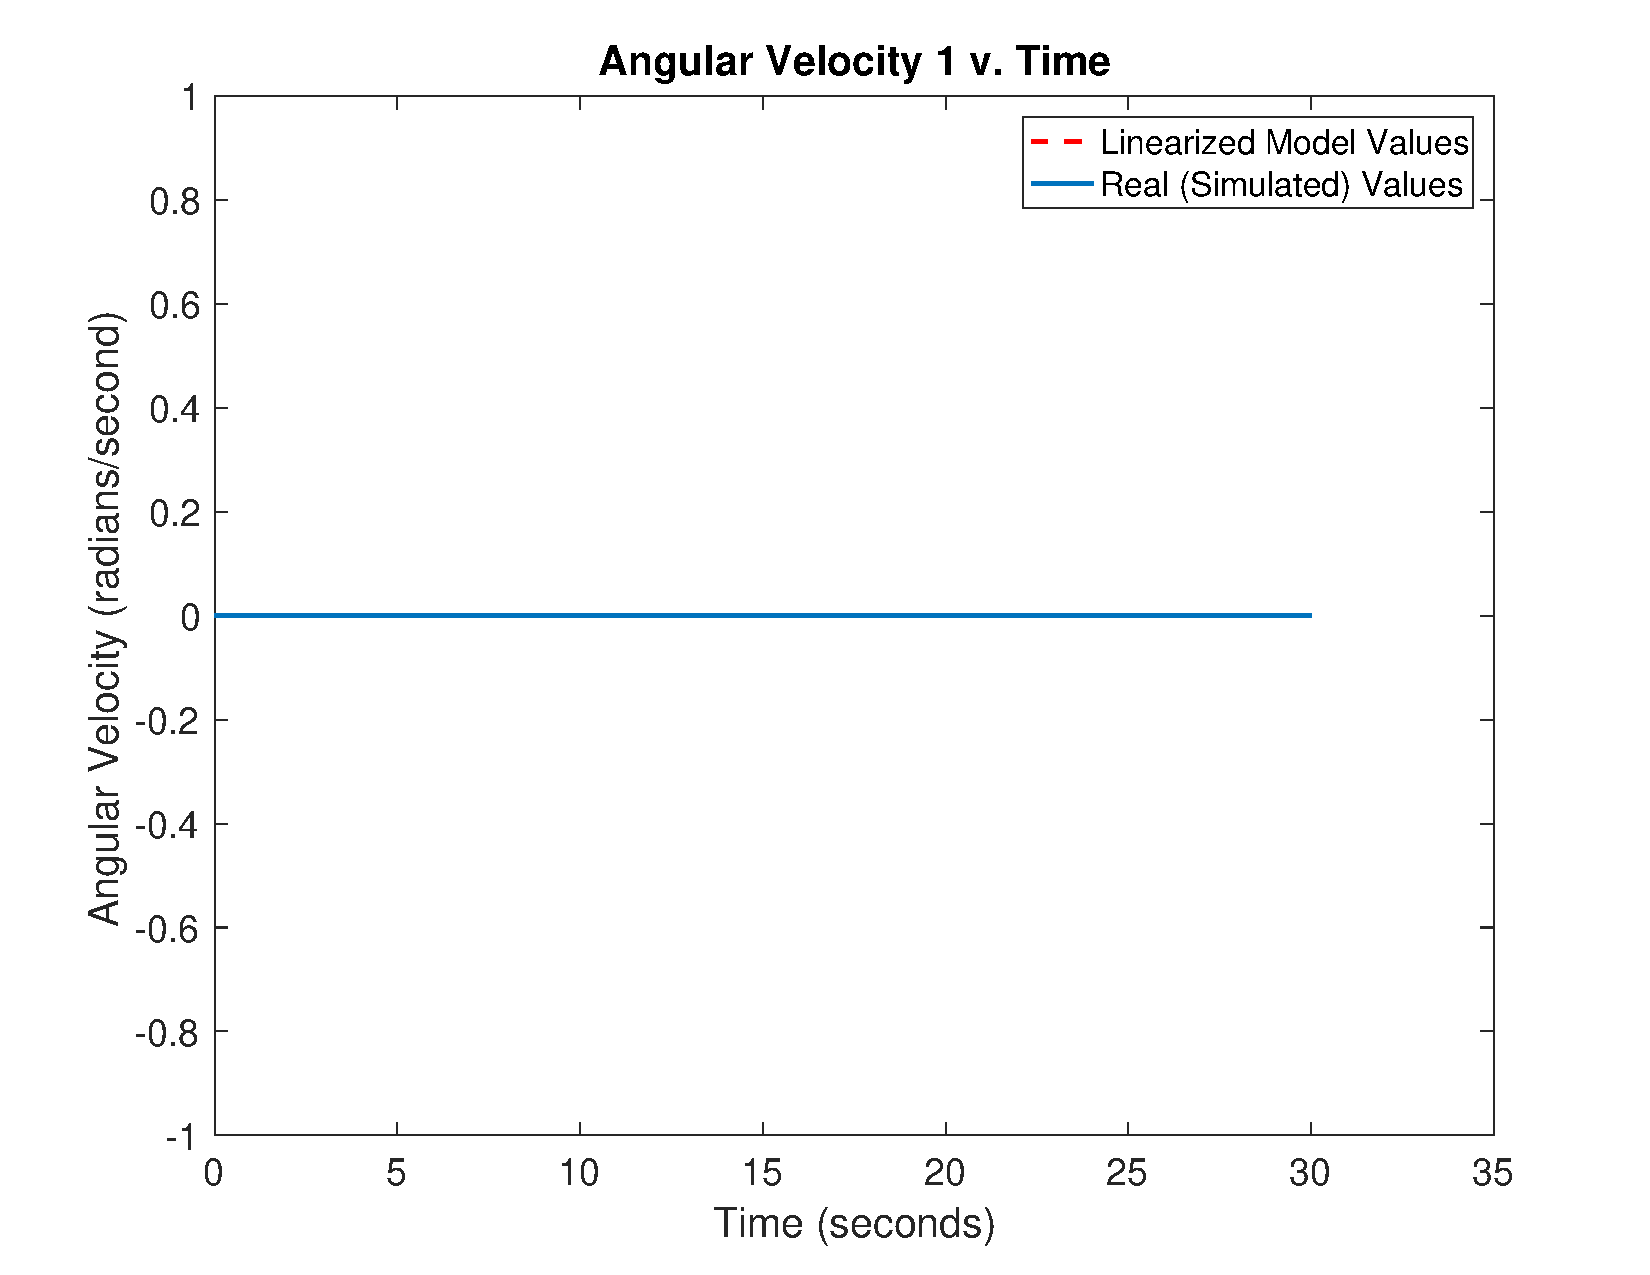
\includegraphics[width=0.35\textwidth]{w1a.pdf}}
\subfloat[$w_{2}$]{
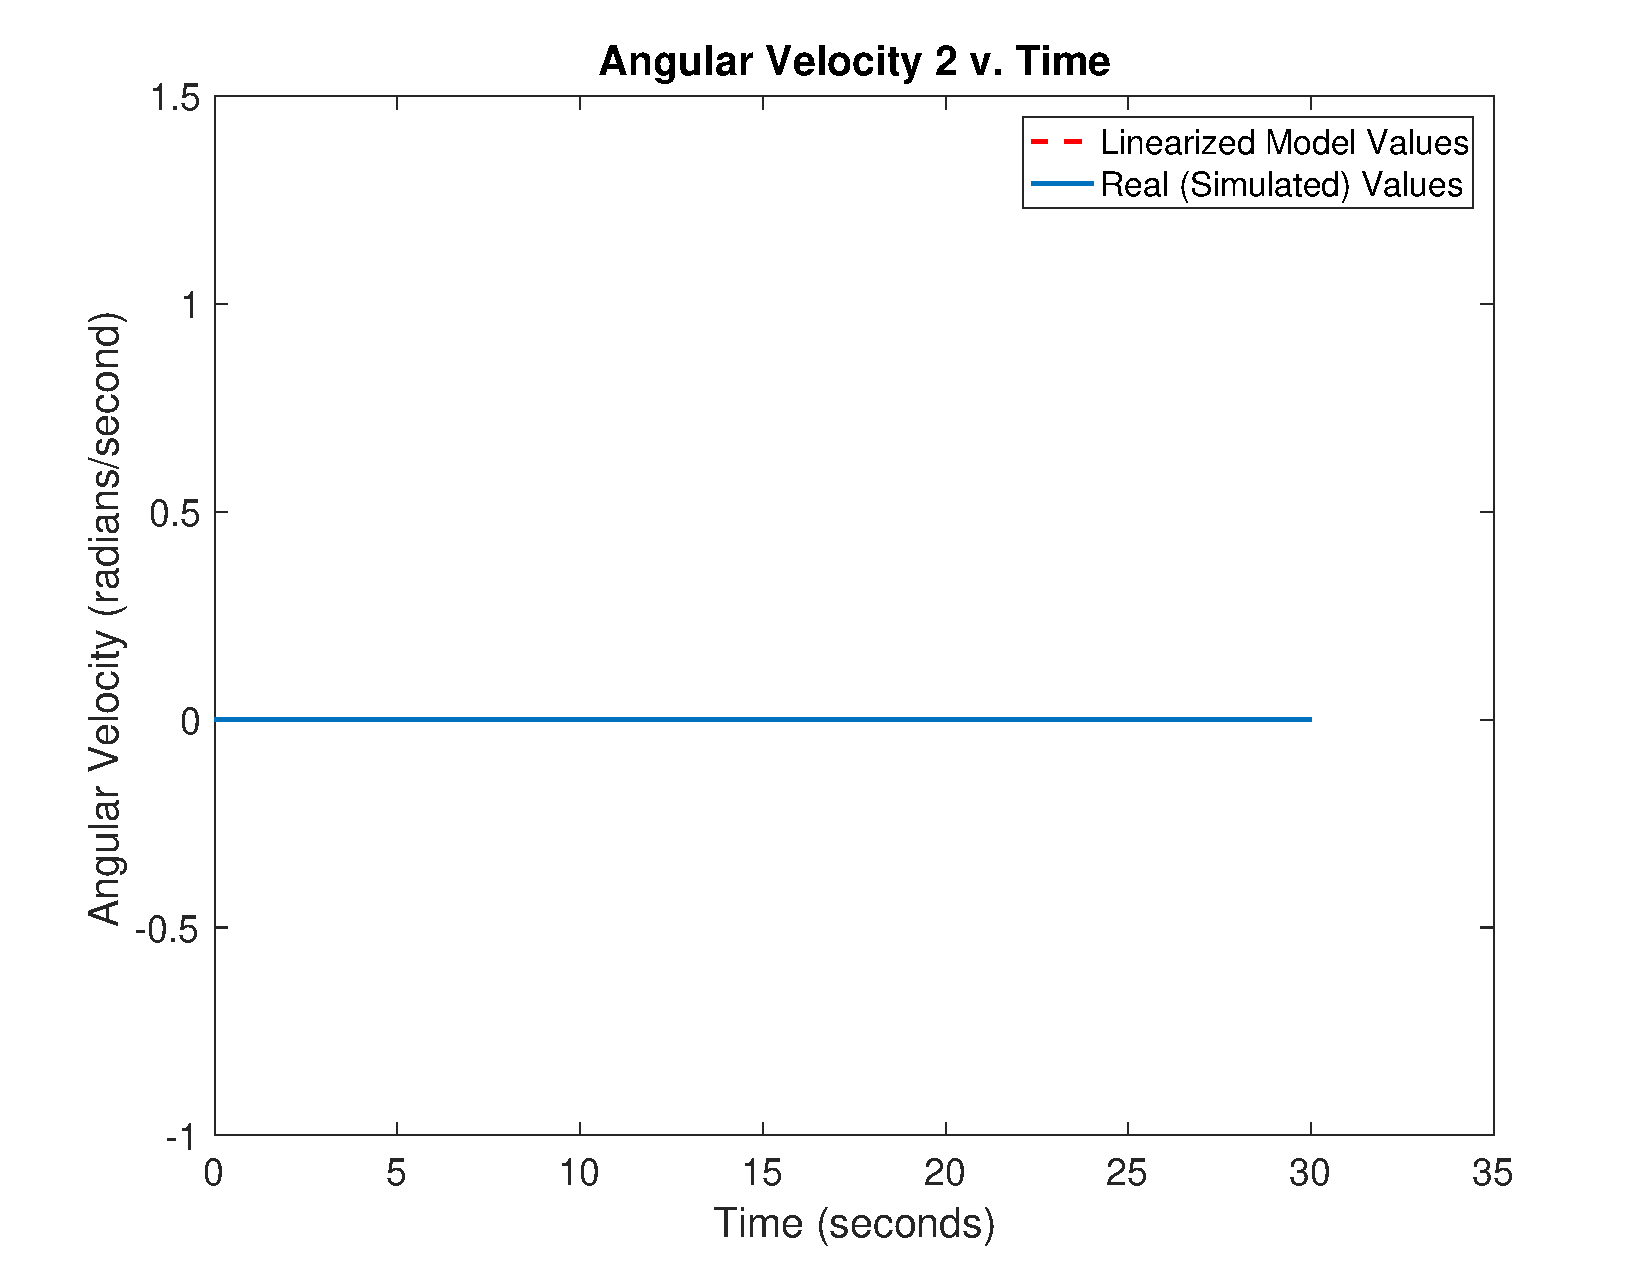
\includegraphics[width=0.35\textwidth]{w2a.pdf}}
\subfloat[$w_{3}$]{
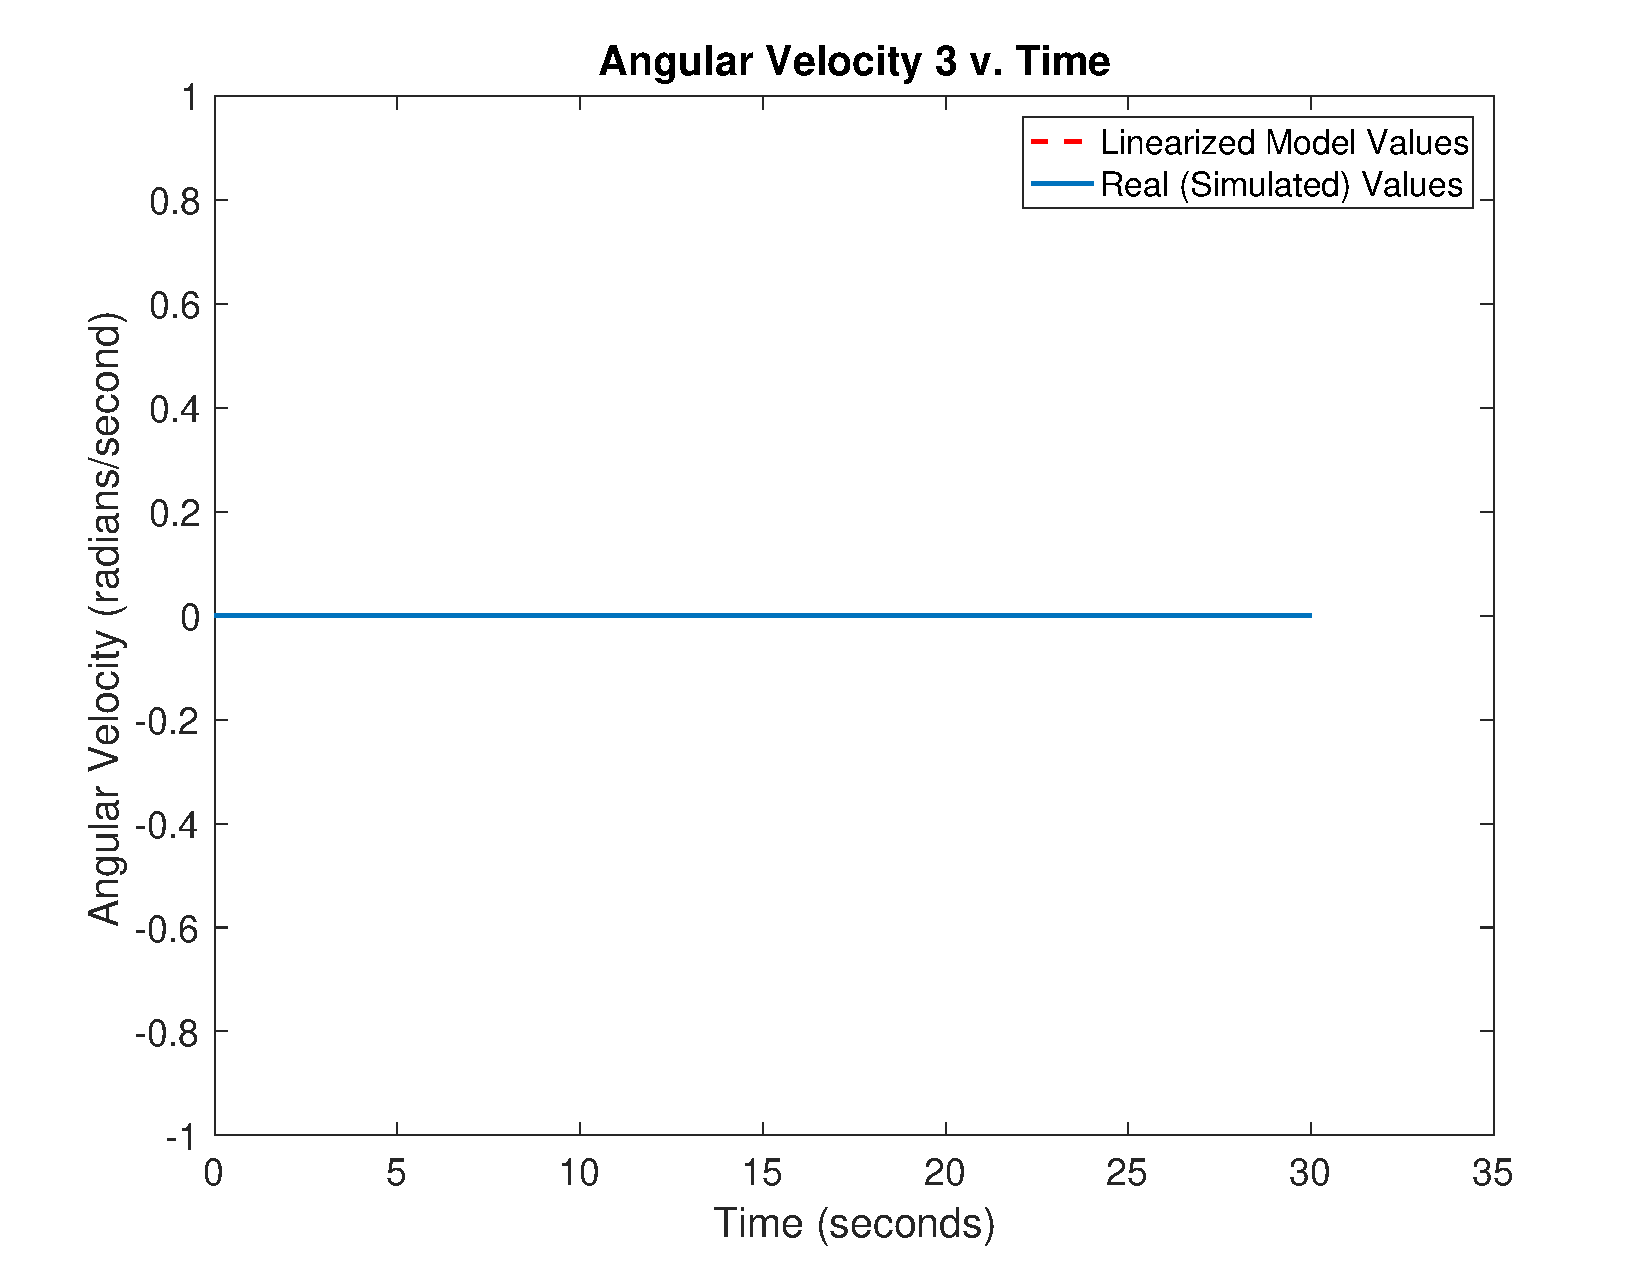
\includegraphics[width=0.35\textwidth]{w3a.pdf}}
\caption{The linear and nonlinear system for $w_{1}$, $w_{2}$, $w_{3}$ when $w_{0} = w_{e}$}
\label{fig:1}
\end{figure}
\clearpage
\vspace{5mm}
If the nonlinear system has initial conditions equal to the equilibrium point, the resulting plot will have strong similarities between the nonlinear system and the linear system. Represented in Figure \ref{fig:1} exist a simulation where the initial conditions are equivalent to the equilibrium point, $w_{0} = w_{e}$. If the initial conditions were to differ slightly from the equilibrium point, noticeable differences will be seen between the two systems. 
\begin{figure}[h!]
\centering
\subfloat[$w_{1}$ ]{
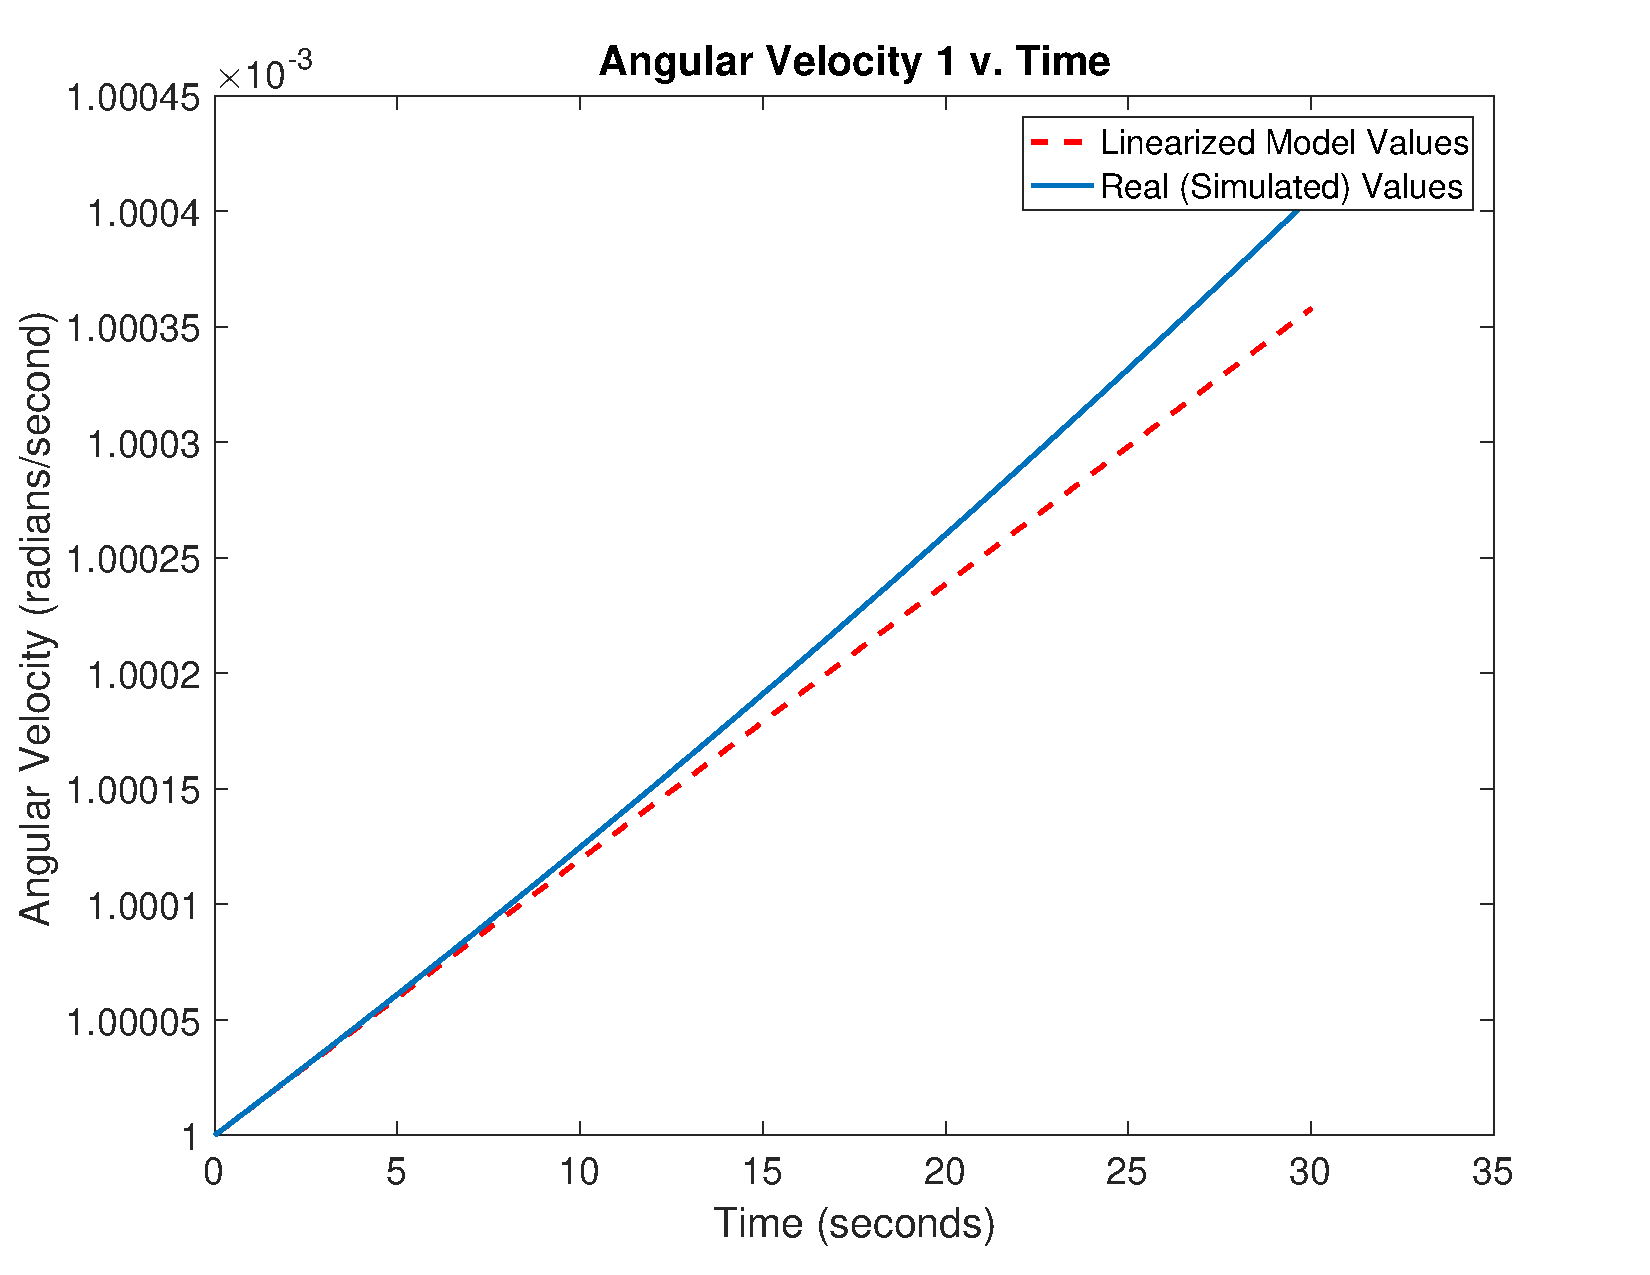
\includegraphics[width=0.35\textwidth]{w1b.pdf}}
\subfloat[$w_{2}$]{
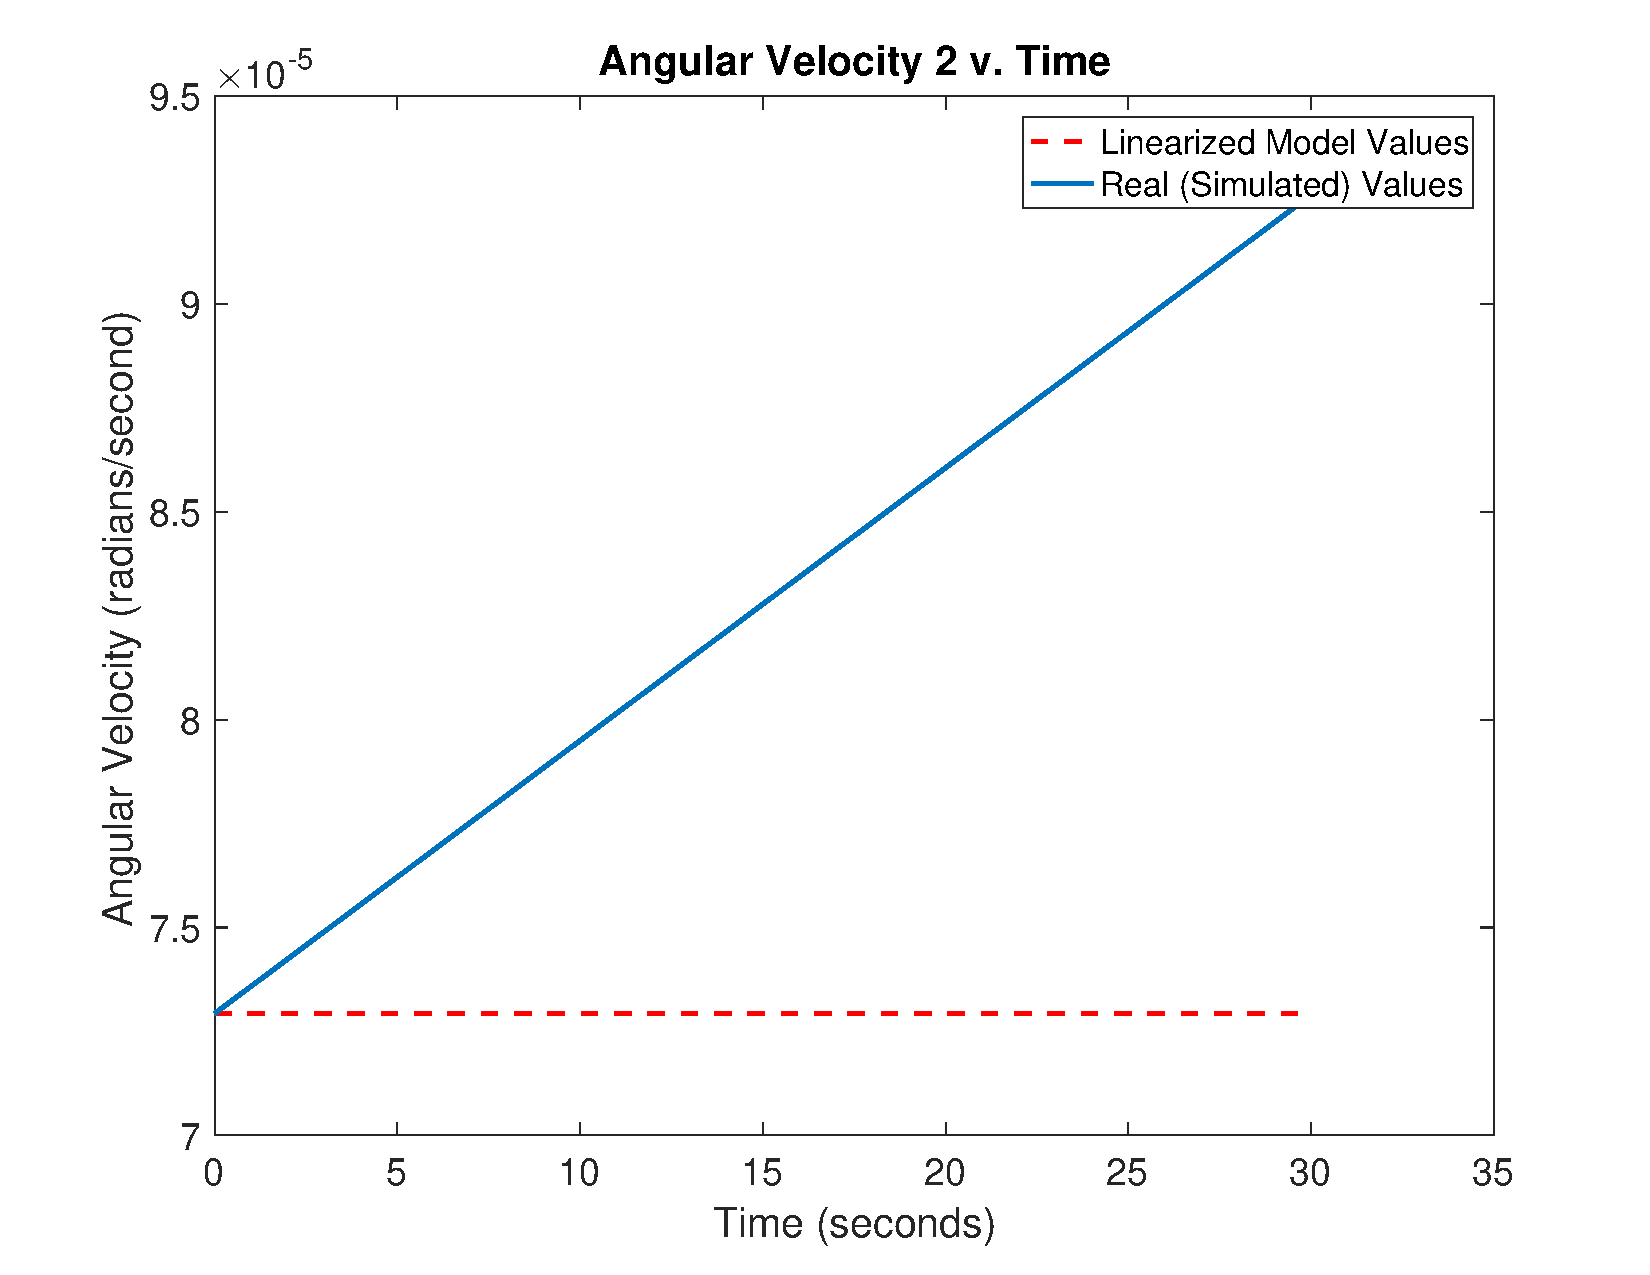
\includegraphics[width=0.35\textwidth]{w2b.pdf}}
\subfloat[$w_{3}$]{
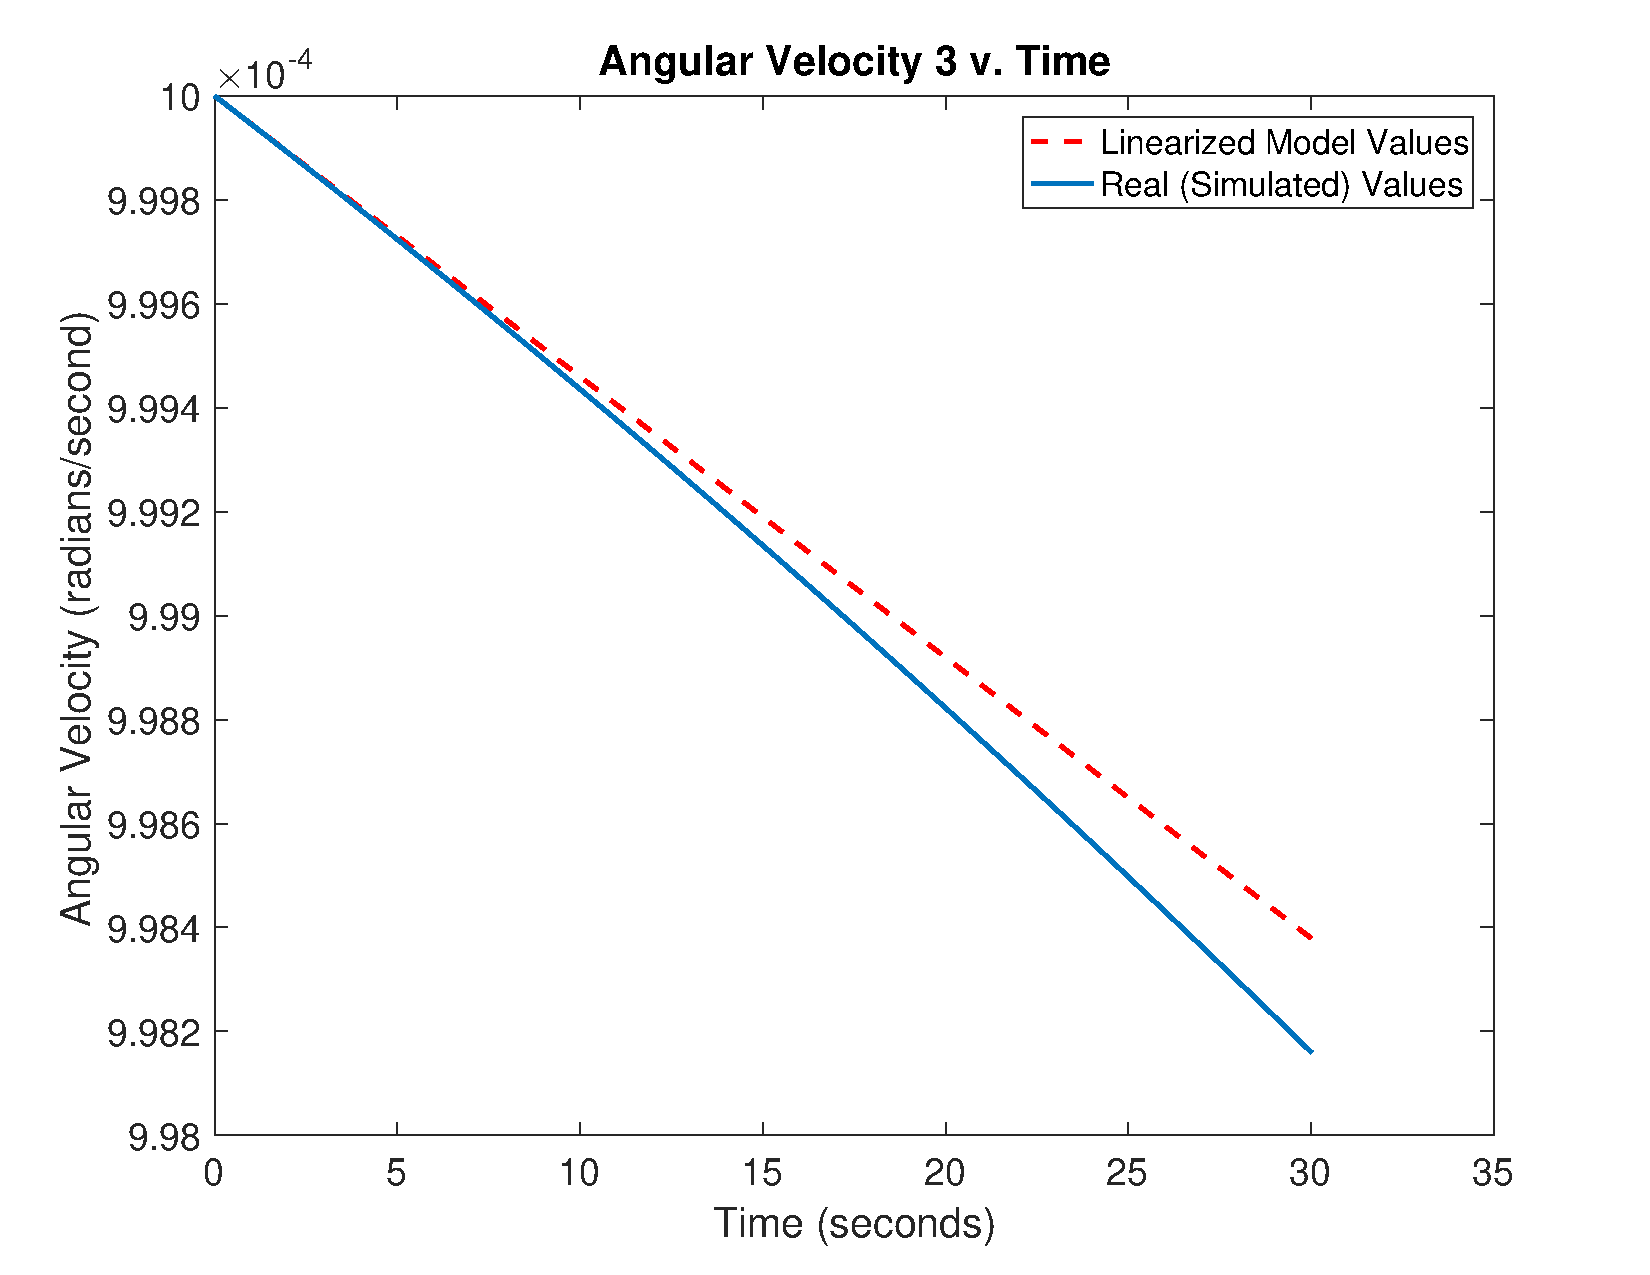
\includegraphics[width=0.35\textwidth]{w3b.pdf}}
\caption{The linear and nonlinear system for $w_{1}$, $w_{2}$, $w_{3}$ when $w_{0} = 0.01w_{e}$}
\label{fig:2}
\end{figure}
\\
In Figure \ref{fig:2} it is shown how with a $.1\%$ increase to the initial values, the nonlinear system begins to differ from the linear model.
\begin{figure}[h!]
\centering
\subfloat[$w_{1}$ ]{
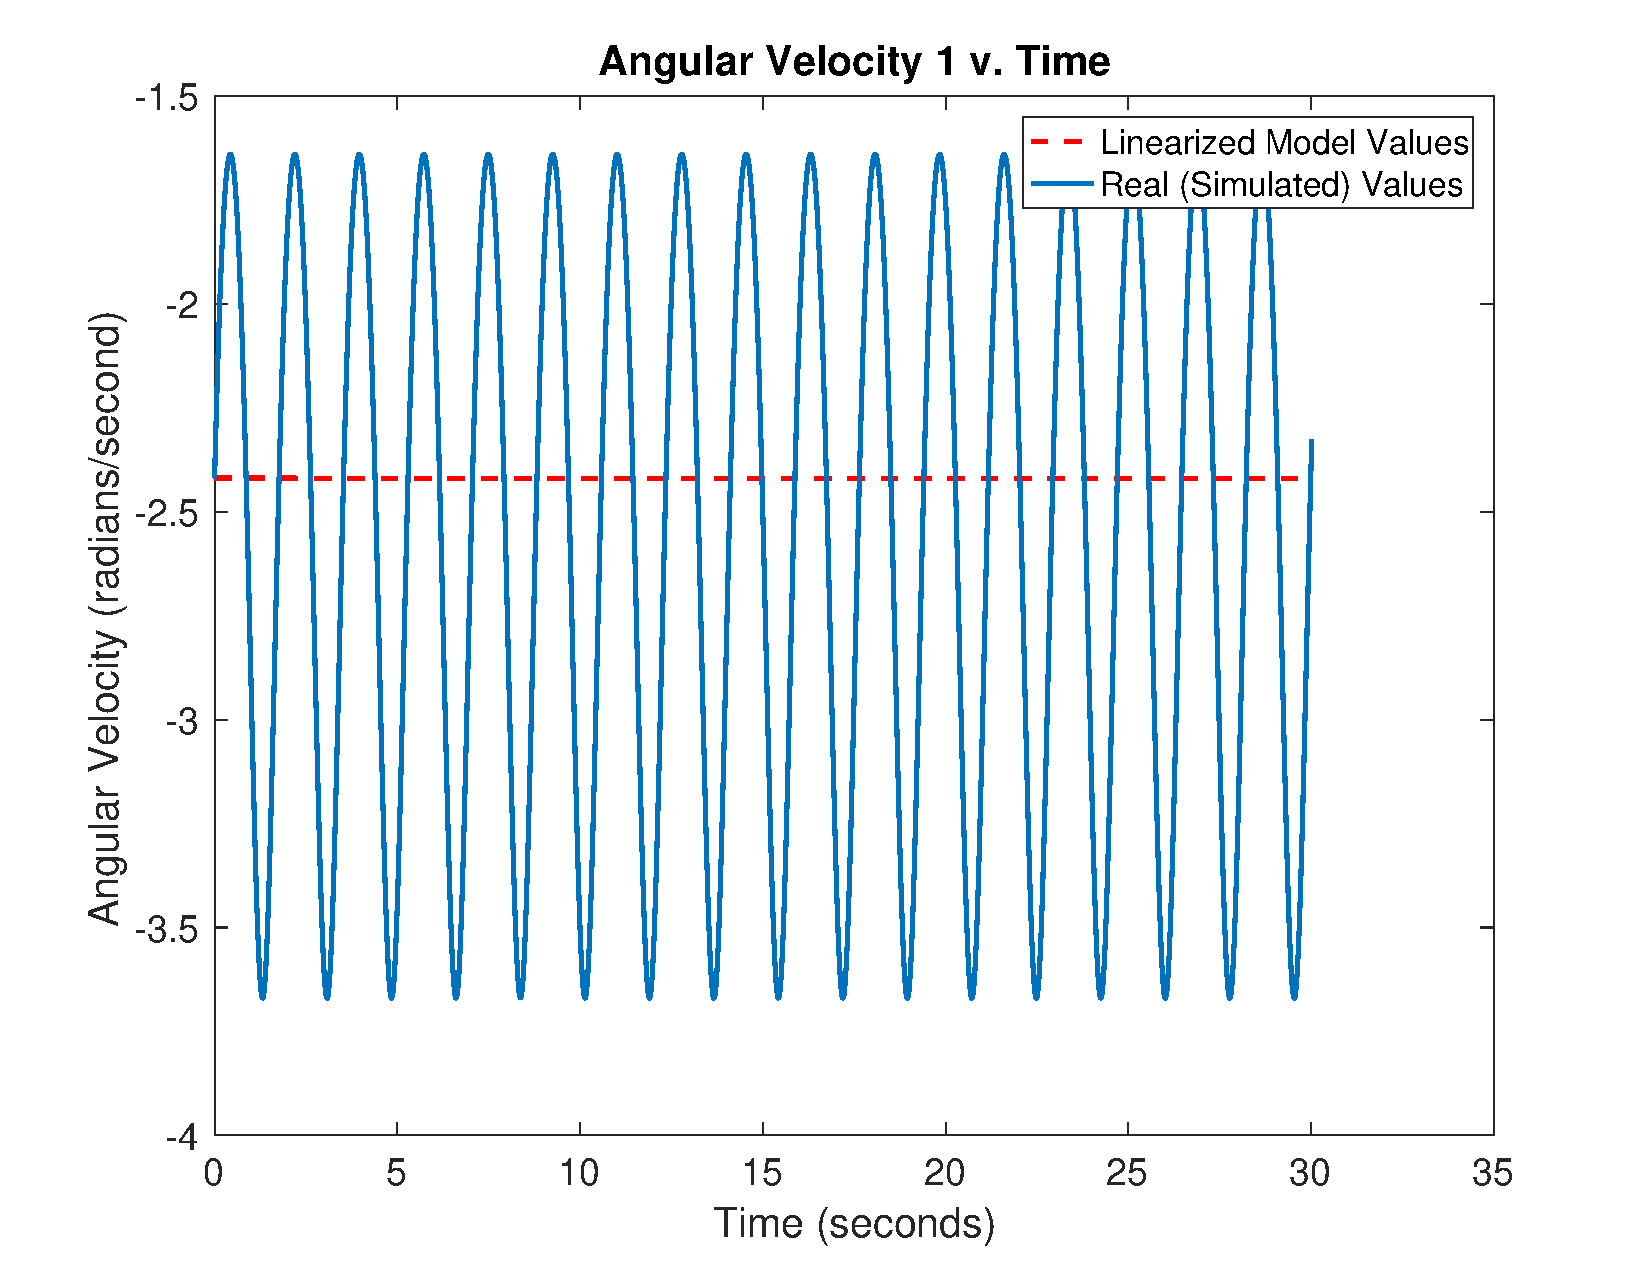
\includegraphics[width=0.35\textwidth]{w1c.pdf}}
\subfloat[$w_{2}$]{
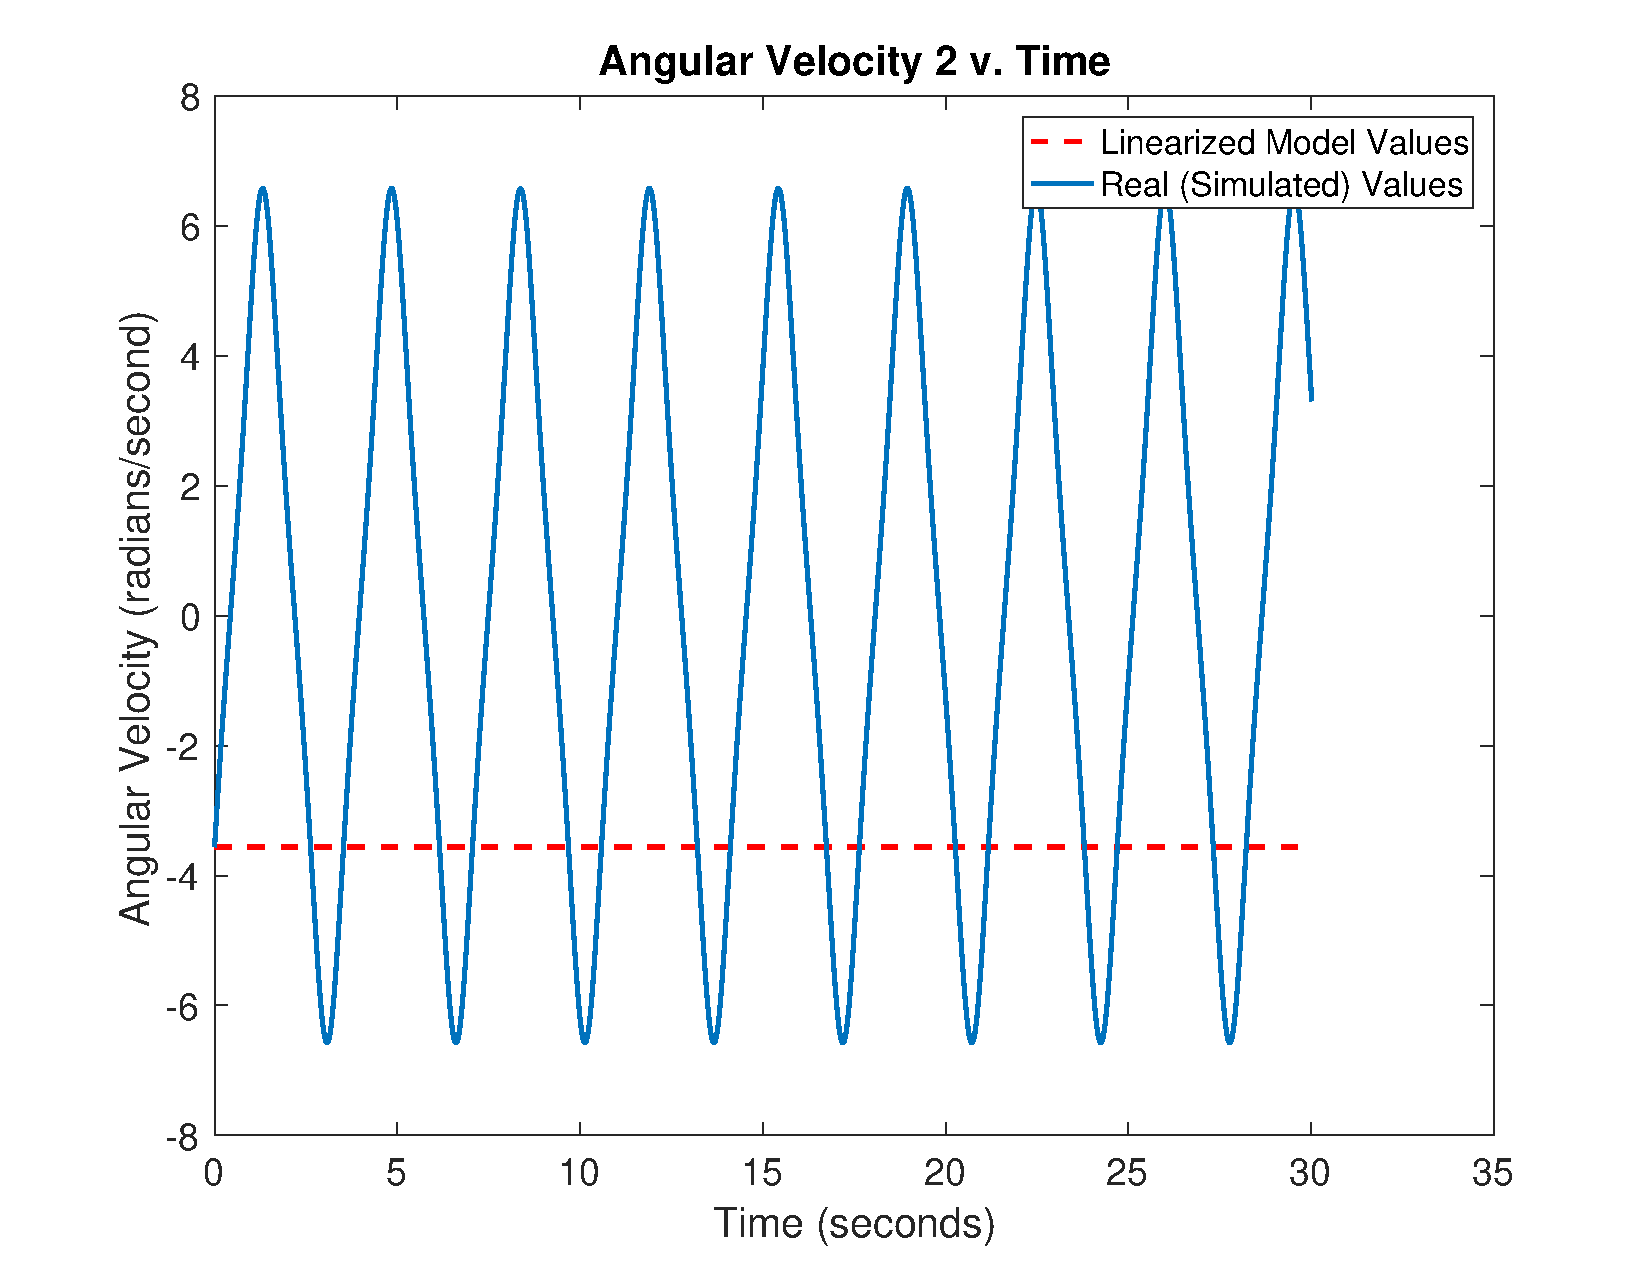
\includegraphics[width=0.35\textwidth]{w2c.pdf}}
\subfloat[$w_{3}$]{
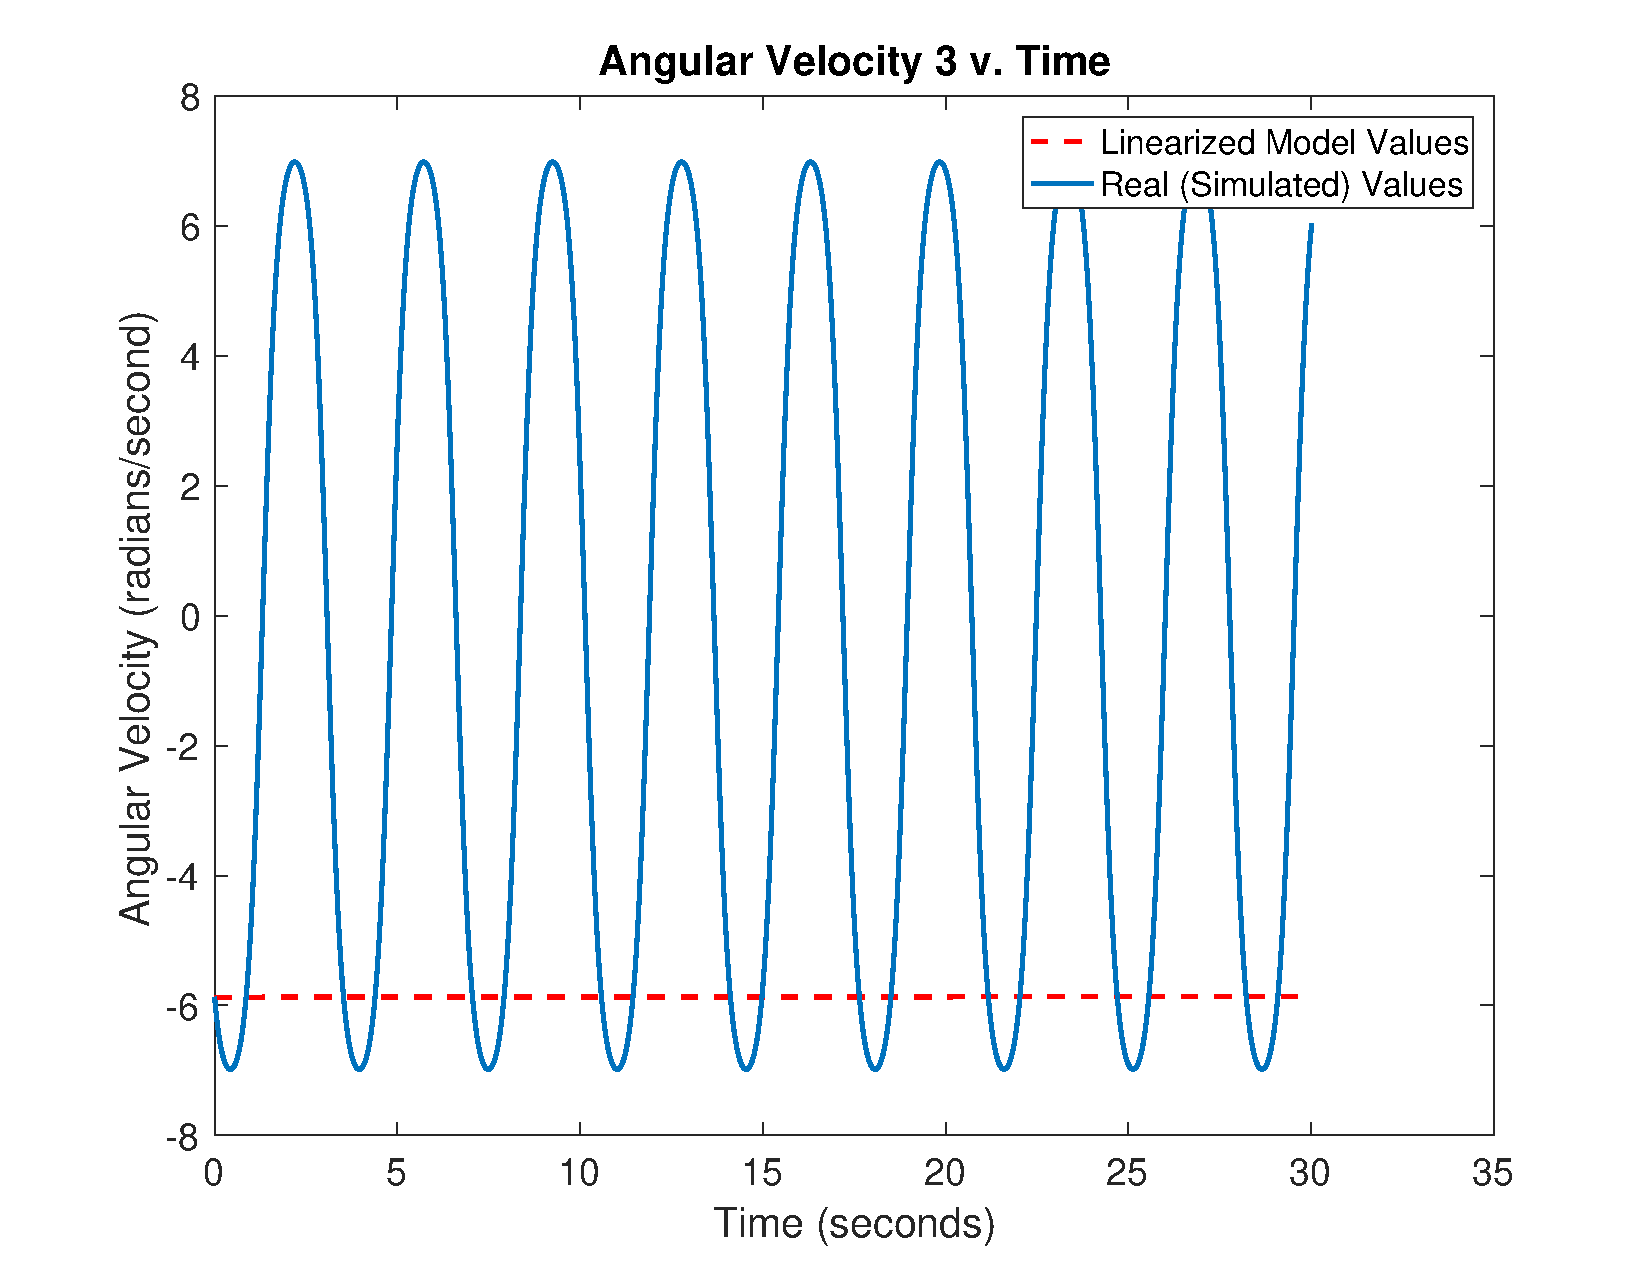
\includegraphics[width=0.35\textwidth]{w3c.pdf}}
\caption{The linear and nonlinear system for $w_{1}$, $w_{2}$, $w_{3}$ when $w_{0} = rand(w_{e})$}
\label{fig:3}
\end{figure}
\\ \\
The further away the initial angular velocity is from the equilibrium point, the less accurate the linear model will be as shown in Figure \ref{fig:3}. Since Figure \ref{fig:1} shows an identical relation between the linear and nonlinear model, the accuracy of the linear model is verified. This will prove to be very useful when state feedback is applied.
\clearpage
\section{State Feedback}
The next step in the evolution of the state-space model is to introduce state feedback. State feedback is defined as a system in which the input depends on the state. State feedback has the input
\begin{align}
\label{eqn7}
u = -Kx
\end{align}
In equation \ref{eqn7}, $K$ represents a constant matrix whose values can be defined and manipulated to achieve equilibrium. The way in which state feedback,$u=-Kx$, differs from zero input response, $u=0$, is through the inputs ability to change. Previously, the system would remain at its initial conditions for angular velocity since no torque was being applied to the craft. However, with a state feedback input, this is no longer the case. Torque is now applied to the craft and with a proper formulation of $K$ the system can converge to the desired equilibrium points. 
\\ \\ 
In this system, the defined input is $u=-Kx$ for all instances of $t$. The resulting state-space system is
\begin{align*}
\dot{x} &= (A-BK)x \\
y &= Cx
\end{align*}
This state-space model will have the solution
\begin{equation}
\begin{aligned}
x_{t} &= e^{(A-Bk)t}x_{0} \\
y_{t} &= Ce^{(A-Bk)t}x_{0}
\end{aligned}
\end{equation}
With the choice of $u$ to be a state feedback model, the actuators will now apply some torque proportional to the chosen value $K$. Since no methodological approach to solving $K$ has been shown, the values for the constants of $K$ are derived using trial and error. An attempt at a methodology known as "Pole Placement" for state feedback control  proved unsuccessful. It is known that $K$ must be a 2x3 matrix. This is known by studying the dimensions of the $u$ and $x$ matrix which have a vertical dimension of 2 and a horizontal dimension of 3 respectively. Using this approach, $K$ is found to be
\begin{equation}
K = 
\begin{bmatrix} 
1 & 0 & -1
\\
-1 & 1 & 0
\end{bmatrix}
\end{equation}
By setting K to this value, the angular velocity of the craft will converge to the equilibrium point for initial conditions near equilibrium. In Figure \ref{fig:4}, the initial conditions are set such that $w_{2}$ is increased by a magnitude of 10. The alternative angular velocities were kept at zero so that this instance would only represent the effects K has on the angular velocity $w_{2}$. \clearpage
\begin{figure}[h!]
\centering
\subfloat[t 0:6 seconds]{
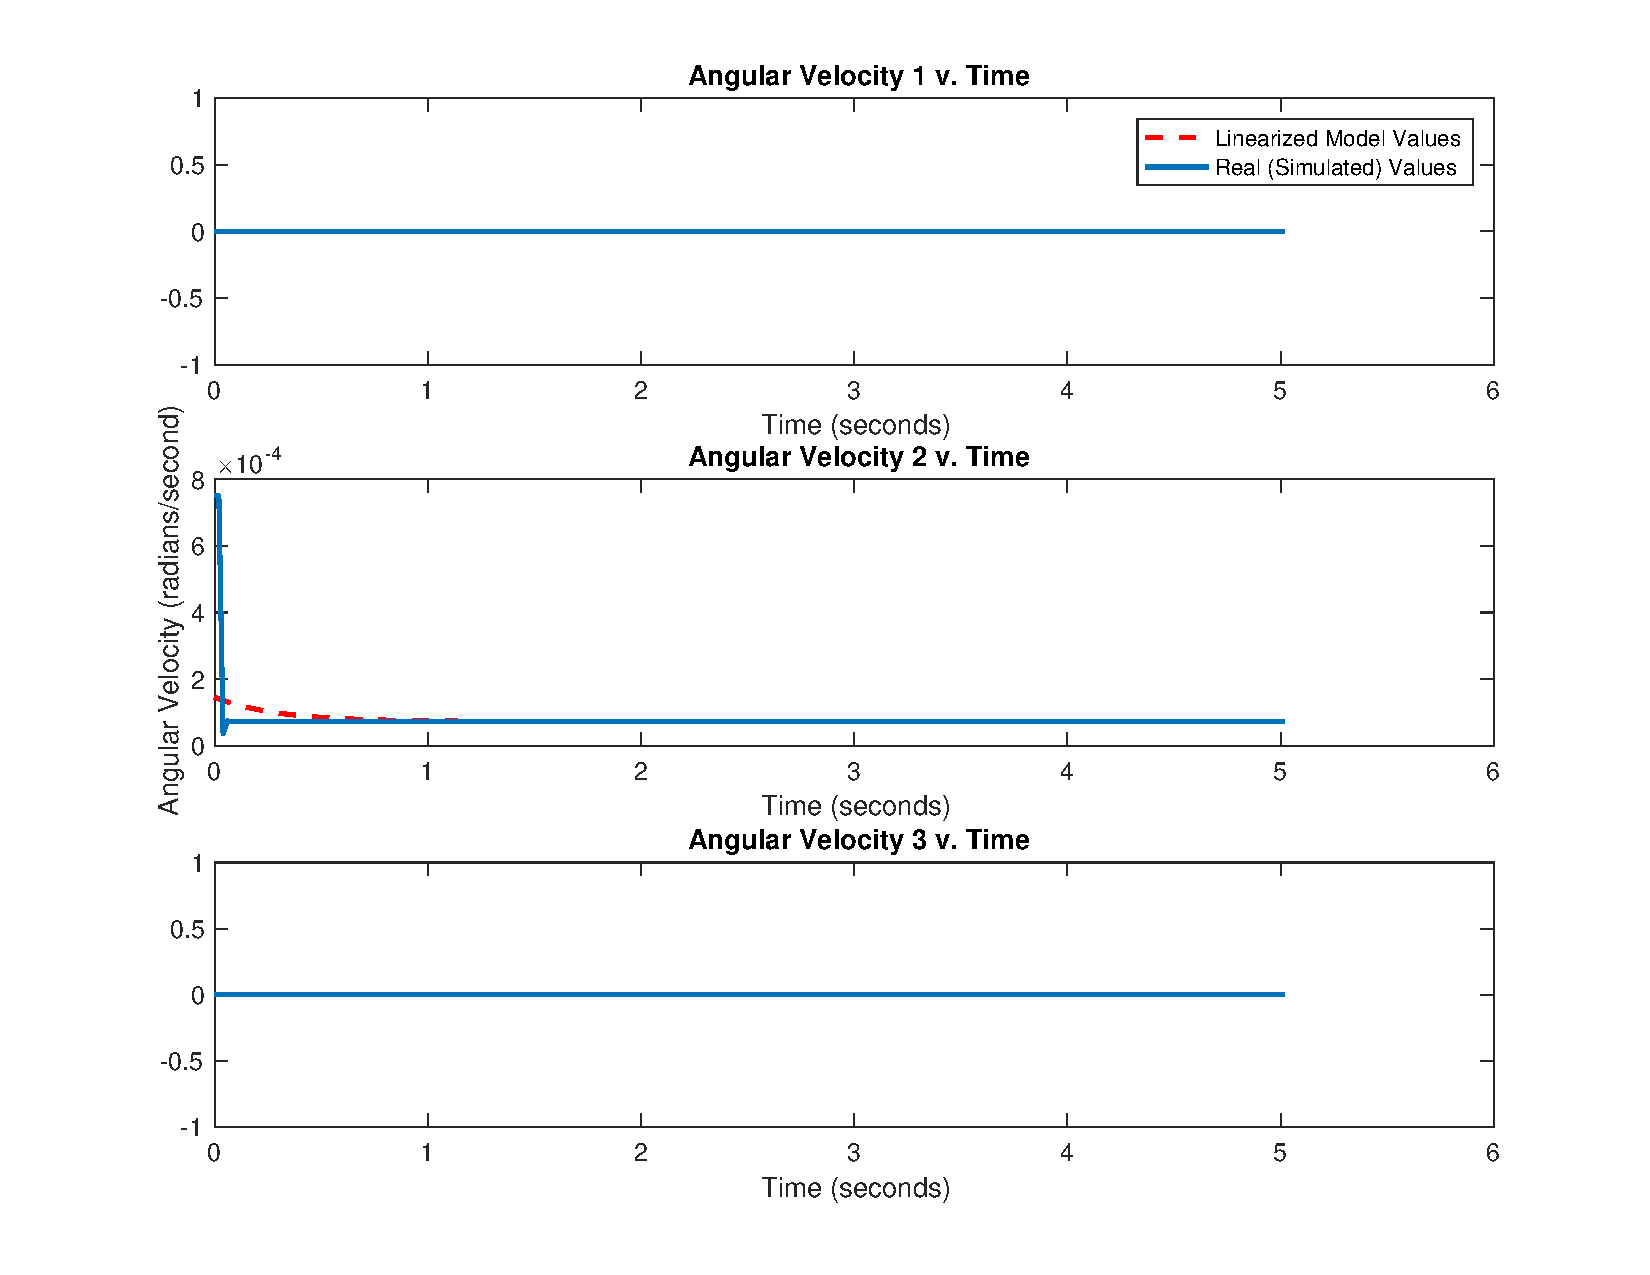
\includegraphics[width=0.5\textwidth]{wall1.pdf}}
\subfloat[t 0:0.5 seconds]{
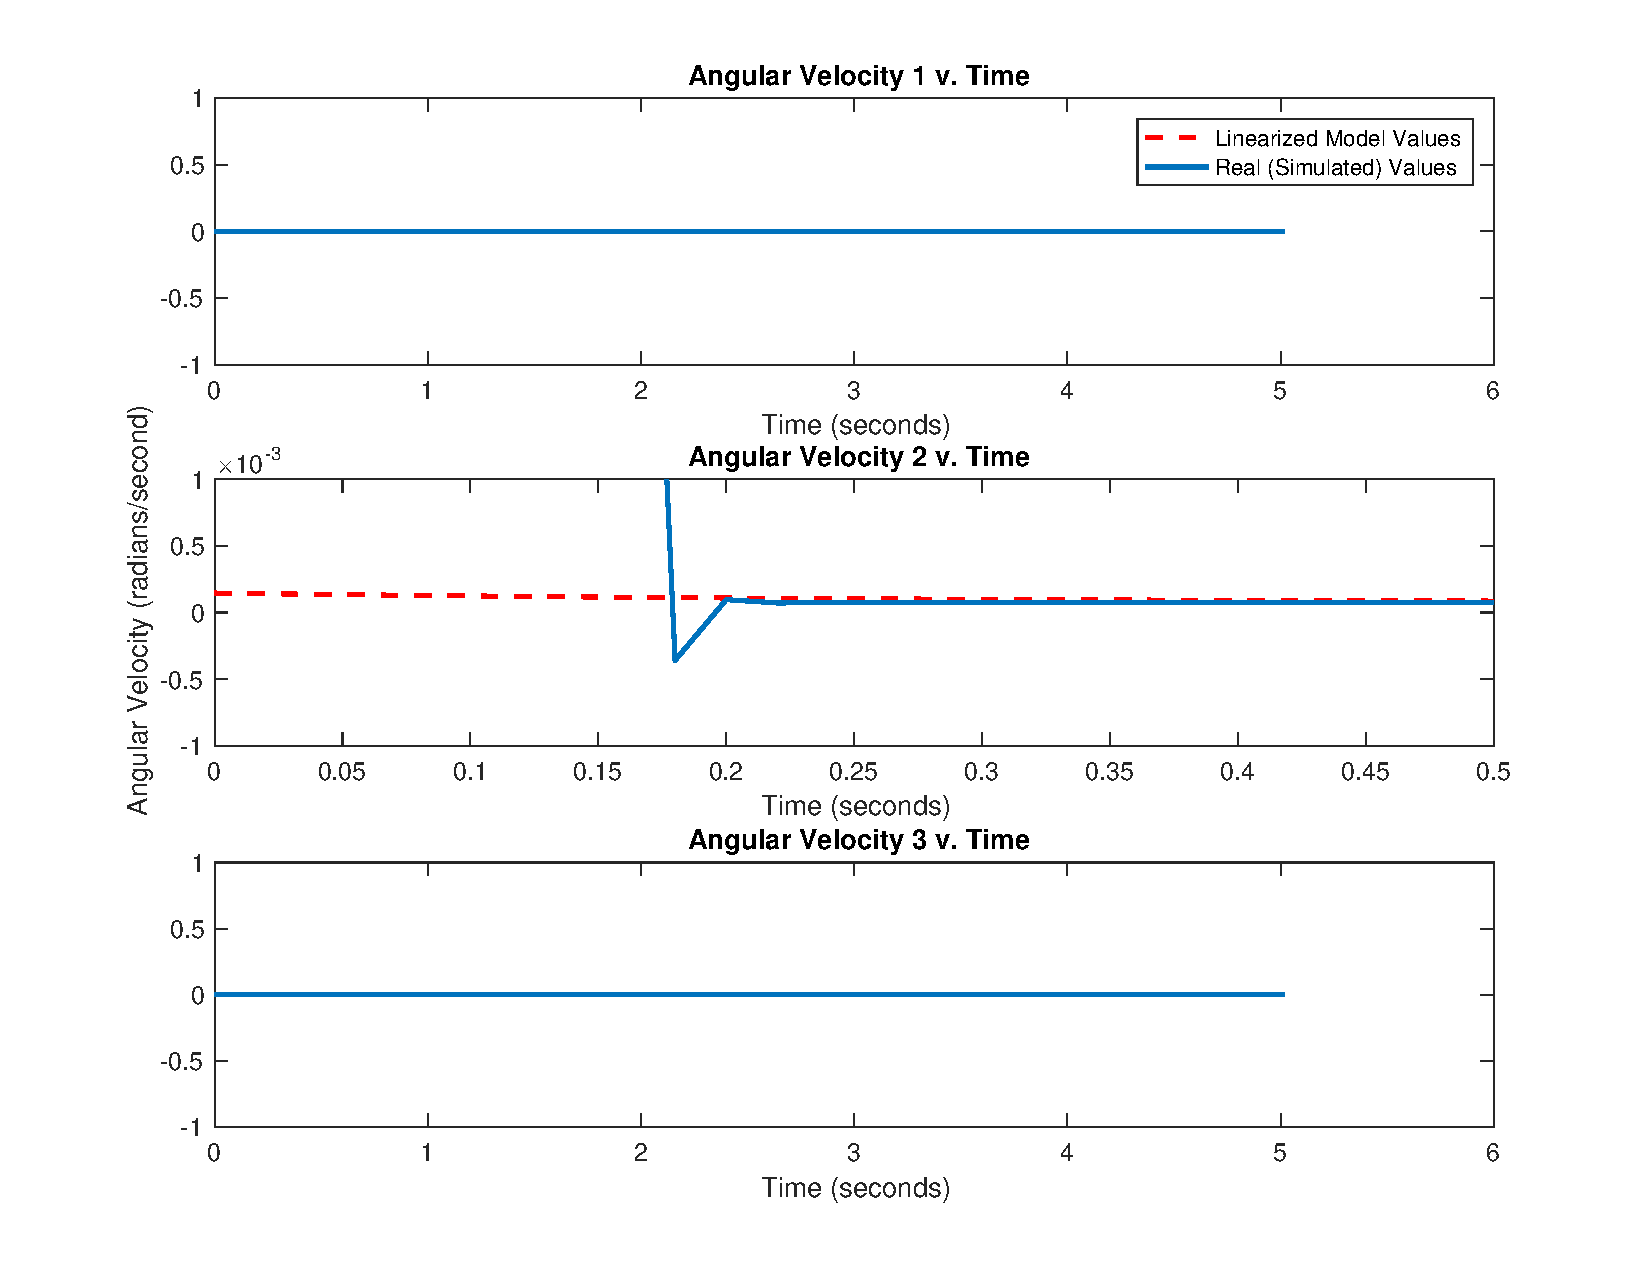
\includegraphics[width=0.5\textwidth]{wall2z.pdf}}
\caption{The linear and nonlinear system for $w_{1}$, $w_{2}$, $w_{3}$ when $w_{0} \approx w_{e}$}
\label{fig:4}
\end{figure}
In Figure \ref{fig:4}, it is visible in "Angular Velocity 2 v. Time" that the real model and linearized model converge at the same place. By analyzing the data, it is confirmed that the two converge to the equilibrium point $we_{2}$. The remaining two plots had an initial angular velocity equal to the equilibrium angular velocity so no change is present. In Figure \ref{fig:5}, the angular velocities $w_{1}$ and $w_{3}$ where changed by adding 0.01.
\begin{figure}[h!]
\centering
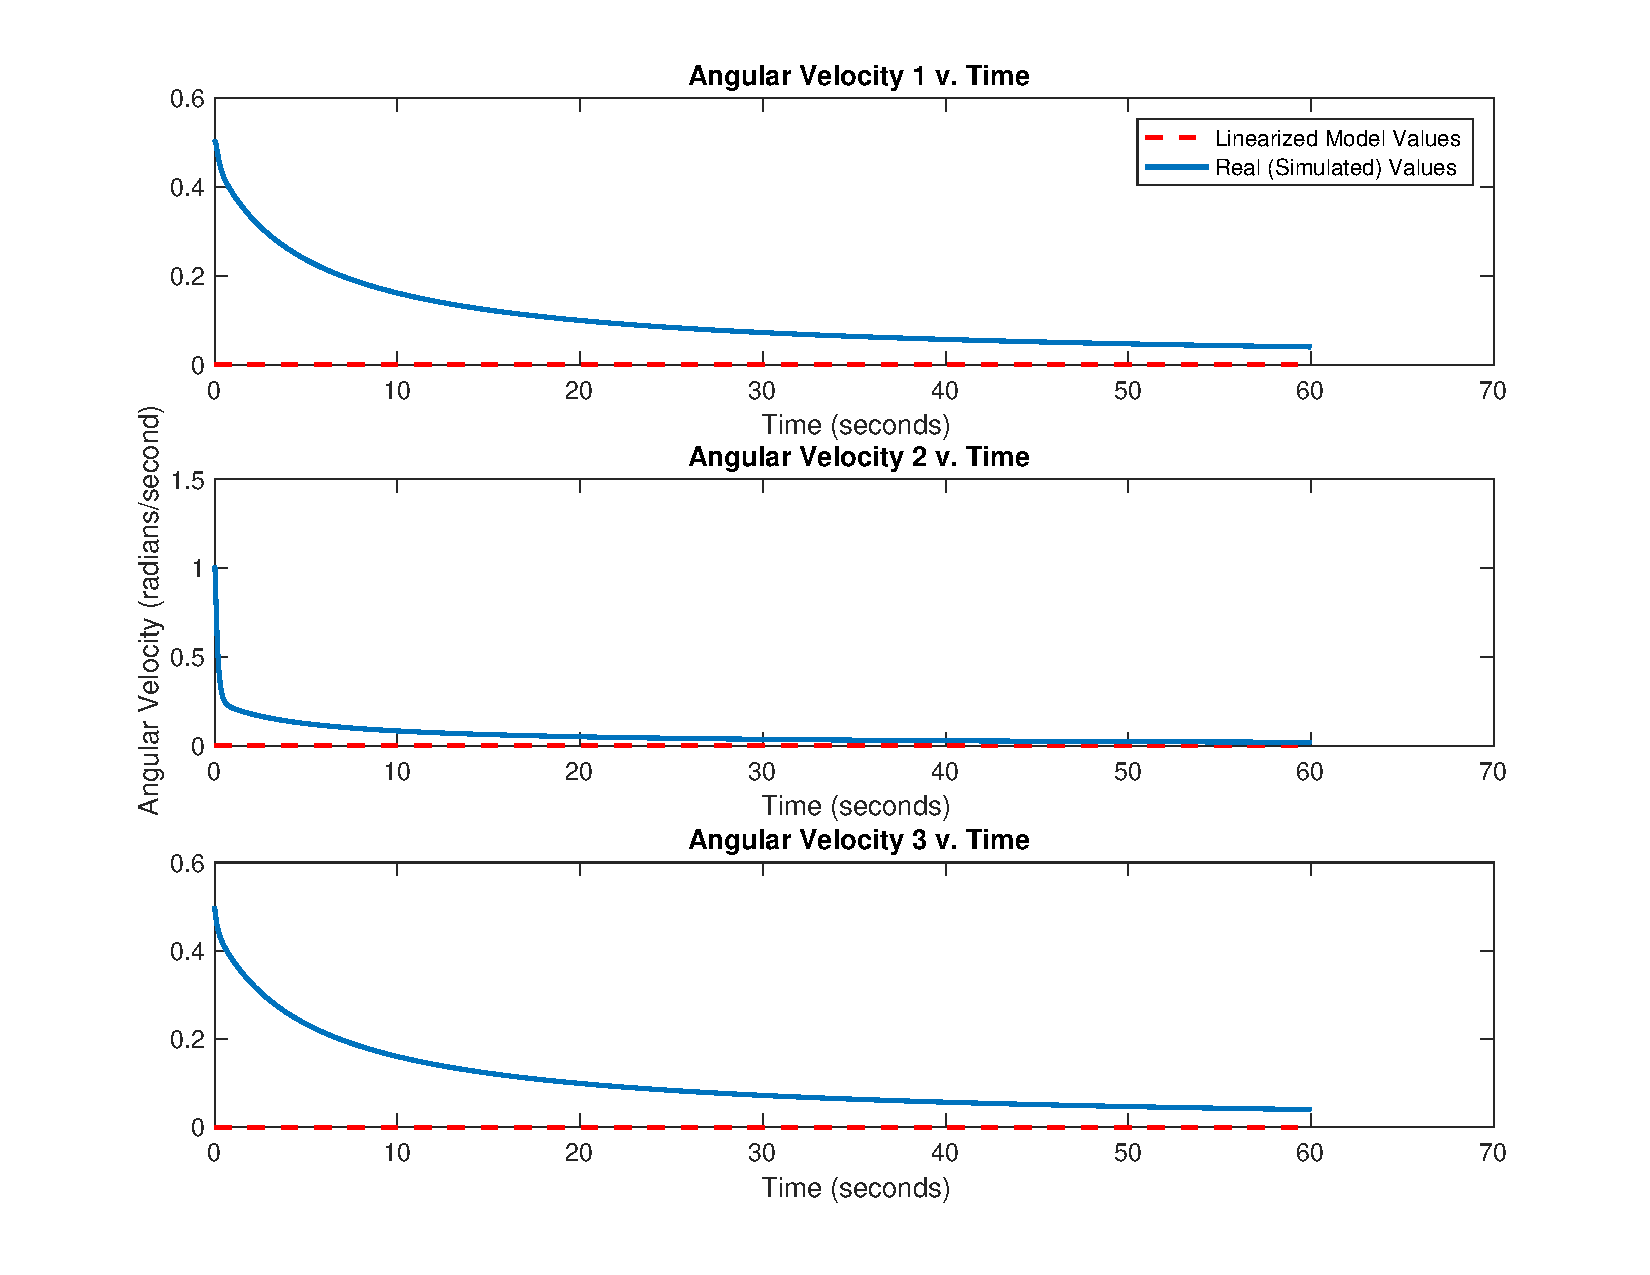
\includegraphics[width=0.6\textwidth]{wall3.pdf}
\caption{The linear and nonlinear system for $w_{1}$, $w_{2}$, $w_{3}$ when $w_{0} > w_{e}$ }
\label{fig:5}
\end{figure}
Once again, the values begin to converge to the desired equilibrium points. Since the values for K were derived using Trial and error, the accuracy of convergence deteriorates as the difference between $w_{0}$ and $w_{e}$ increases. Had a more methodological approach for K been taken, the system error would be expected to be less.
\section{Stability}
For both Zero Input and State Feedback, values of the K matrix were manipulated to achieve a system convergence at equilibrium. An approach to confirming convergence that was used in the above sections was interpretation of eigenvectors and eigenvalues. This process is simplified through the use of technology. For the case of a zero input response, the following input to MATLAB is made
\begin{lstlisting}[frame=single]
[V,F]=eig(A) %Zero Input
\end{lstlisting}
For the case of state feedback, the following input to MATLAB is made
\begin{lstlisting}[frame=single]
[V,F]=eig(A-B*K) %State Feedback
\end{lstlisting}
Where A, B and K are all predefined matrices for the state-space model. The term for which the eigenvector and eigenvalues is taken from is the term dependent on the state of the system as shown in Equation \ref{eqn10} as $A$ or $(A-BK)$
\begin{equation}
\label{eqn10}
\dot{x} = Ax
\qquad
\dot{x} = (A-BK)x
\end{equation}
After computing the MATLAB function, the matrices $V$ and $F$ are created. The matrices are structured such that the diagonal entries of $F$ are the eigenvalues of $A$ or $A-BK$.  These eigenvalues are denoted by $s_1$, $s_2$, $\hdots$, $s_n$, such that
\\
\begin{equation*}
F = 
\begin{bmatrix}
s_1 & 0 & \hdots & 0 \\
0 & s_2 & \hdots & 0 \\
\vdots & & \ddots & \vdots \\
0 & 0 & \hdots & s_n
\end{bmatrix}.
\end{equation*}
From this, it is found that the exponential of $F t$ produces the result
\begin{equation*}
e^{Ft}  =
\begin{bmatrix}
e^{s_1 t} & 0 & \hdots & 0 \\
0 & e^{s_2 t} & \hdots & 0 \\
\vdots & & \ddots & \vdots \\
0 & 0 & \hdots & e^{s_n t}
\end{bmatrix}.
\end{equation*}
The exponential establishes that the behavior of $x(t)$ is dependent on the entries in the matrix $e^{Ft}$. Two relations can be seen as a result
\begin{itemize}
  \item If $s_1$ is a positive real number, then $e^{s_1 t}$ grows exponentially as $t$ increases meaning the system is unstable.
  \item If $s_1$ is a negative real number, then $e^{s_1 t}$ decays exponentially to zero as $t$ increases meaning the system is stable.
\end{itemize}
With this information in mind, the decision of K can be made such that the eigenvalues are negative real numbers, allowing the system to be stable. The derived eigenvalues are
\begin{equation*}
F_{ZeroInput}= 
\begin{bmatrix} 
0+0 & 0 & 0
\\
0 & 0 & 0
\\
0 & 0 & 0
\end{bmatrix}
\qquad
F_{StateFeedback}= 
\begin{bmatrix} 
-0.035 & 0 & 0
\\
0 & -11.9 & 0
\\
0 & 0 & -5.4*10^{-5}
\end{bmatrix}
\end{equation*}
\section{Reference Tracking}
In Section 6, "State Feedback", it was seen that by choosing an input of $u=-Kx$ with an appropriate K, the system would approach equilibrium as time approaches infinity. With the implementation of reference tracking, the input is made to be linear to the reference point $r$. 
\\
\begin{equation}
\label{eqn11}
u = -K x + k_{ref} r
\end{equation}
Which can be substituted into the state-space model to produce
\begin{equation}
\label{eqn12}
\dot{x} = (A-BK)x + B k_{ref} r
\qquad
y = Cx
\end{equation}
Reference tracking introduces two new terms into the input equation, $k_{ref}$ and $r$. The value for $r$ represents the "reference." It chosen such that as $t \rightarrow \infty$ the value $y \rightarrow r$. For the purposes of achieving the aforementioned goal, r is set to the equilibrium values. The value for $k_{ref}$ is calculated such that the system reaches steady state. The definition of these two knew terms is expressed in Equation \ref{eqn13}.
\begin{equation}
\label{eqn13}
r = \begin{bmatrix} 0 & 7.292115*10^{-5}\end{bmatrix}
\qquad
k_{ref} = \frac{1}{-C(A-BK)^{-1} B}
\end{equation}
\\
It has been established that if the initial conditions were equal to the equilibrium  angular velocities then the system will be stable and experience no changes in torque or angular velocity. In addition, as the initial conditions deviated away from the equilibrium, the system had a more difficult time reaching equilibrium. 
\\ \\
It was observed that with zero input, no change to angular velocity would be made since no torque was being applied to the system. Therefore, once the system left equilibrium, it had no chance of reaching it. 
\\ \\
When observing a state feedback approach, the issue of never returning to equilibrium was resolved. For values close to equilibrium, the system was able to apply an appropriate force to reach some equilibrium. It is important to note however, that the system never truly reached the correct, predefined equilibrium value of $7.292115*10^{-5}$. 
\\ \\ 
By utilizing reference tracking, the system is more likely to reach equilibrium since it is explicitly told to do so. Recall that reference tracking sets $y$ equal to $r$ where $r=w_{e}$. In Figure \ref{fig:6} an initial condition of $w_{0} = [0 1 0]$ was set. Note that the $w_{0,2}$ is significantly larger than the equilibrium value, $w_{0,2} >> w_{e,2}$.
\clearpage
\begin{figure}[h!]
\centering
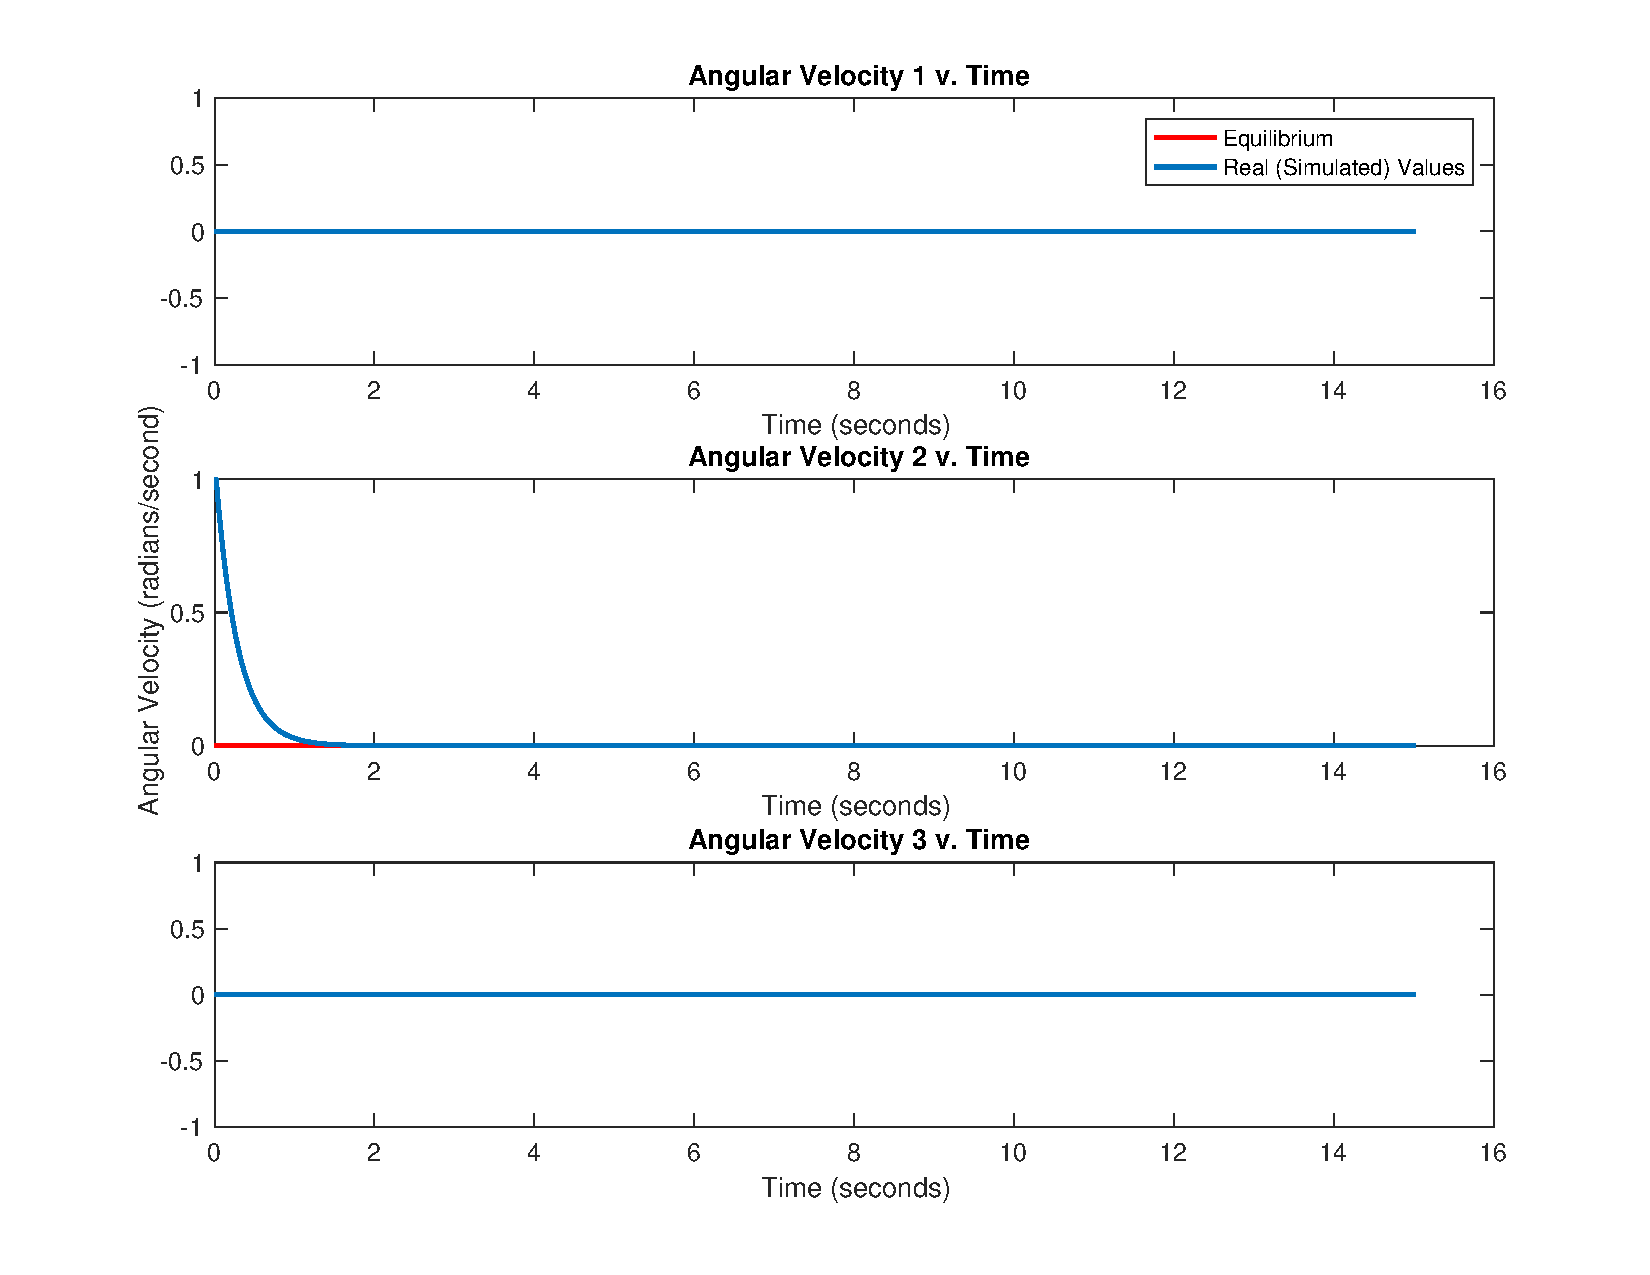
\includegraphics[width=0.5\textwidth]{rt.pdf}
\caption{Spacecraft simulation with  $w_{0}$=[0 1 0]}
\label{fig:6}
\end{figure}
It is visible in the plot and verified in the data that the craft reached equilibrium angular velocity in less than 15 seconds. This is an important distinction to make since when using state feedback, it took 60 seconds to reach a value close to equilibrium. In Figure \ref{fig:7}, the equilibrium is changed such that $w_{0} = [1 1 1]$. It is shown that within the first 5 seconds, both $w_{1}$ and $w_{3}$ approach equilibrium and in 30 seconds, $w_{2}$ comes close to it's equilibrium. 
\begin{figure}[h!]
\centering
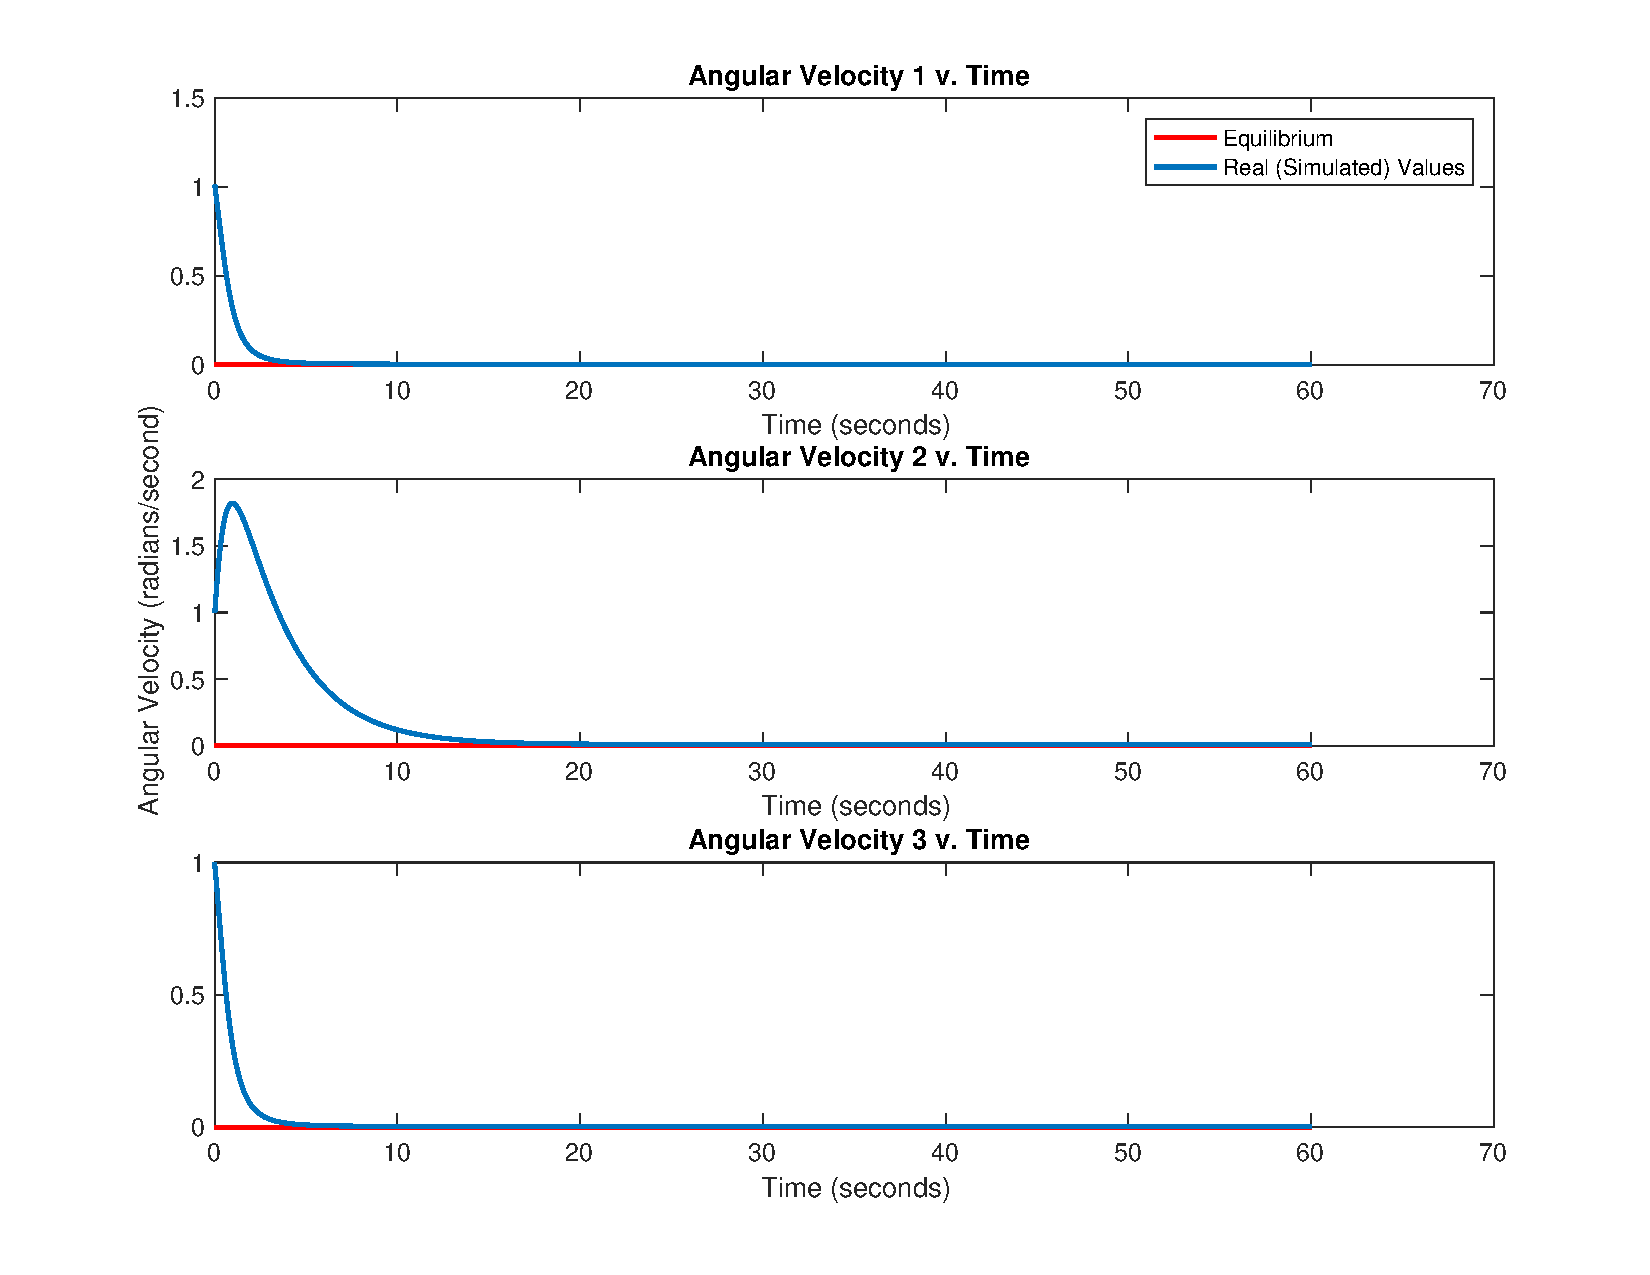
\includegraphics[width=0.5\textwidth]{rt1.pdf}
\caption{Spacecraft simulation with  $w_{0}$=[1 1 1]}
\label{fig:7}
\end{figure}
Finally, three simulations where $w_{0}$ was randomly defined were run. These simulations ran for 600 seconds to increase the chances of equilibrium being reached. It is seen through the plots in Figure \ref{fig:8} that the angular velocities quickly drop to near the equilibrium point within the first 60 seconds but then steadily creep to equilibrium for the remaining time. This has to do with the decision of K. By varying the values of matrix K, different long-term behavior can be seen. Since K can not be methodologically determined at this time, a perfect system cannot be solved for. However, through trail and error, the most fitting K was found to be 
\begin{equation}
K=
\begin{bmatrix}
1 & 0 & -1\\ -0.5 & 0.01 & 0
\end{bmatrix}
\end{equation}


\begin{figure}[h!]
\centering
\subfloat[]{
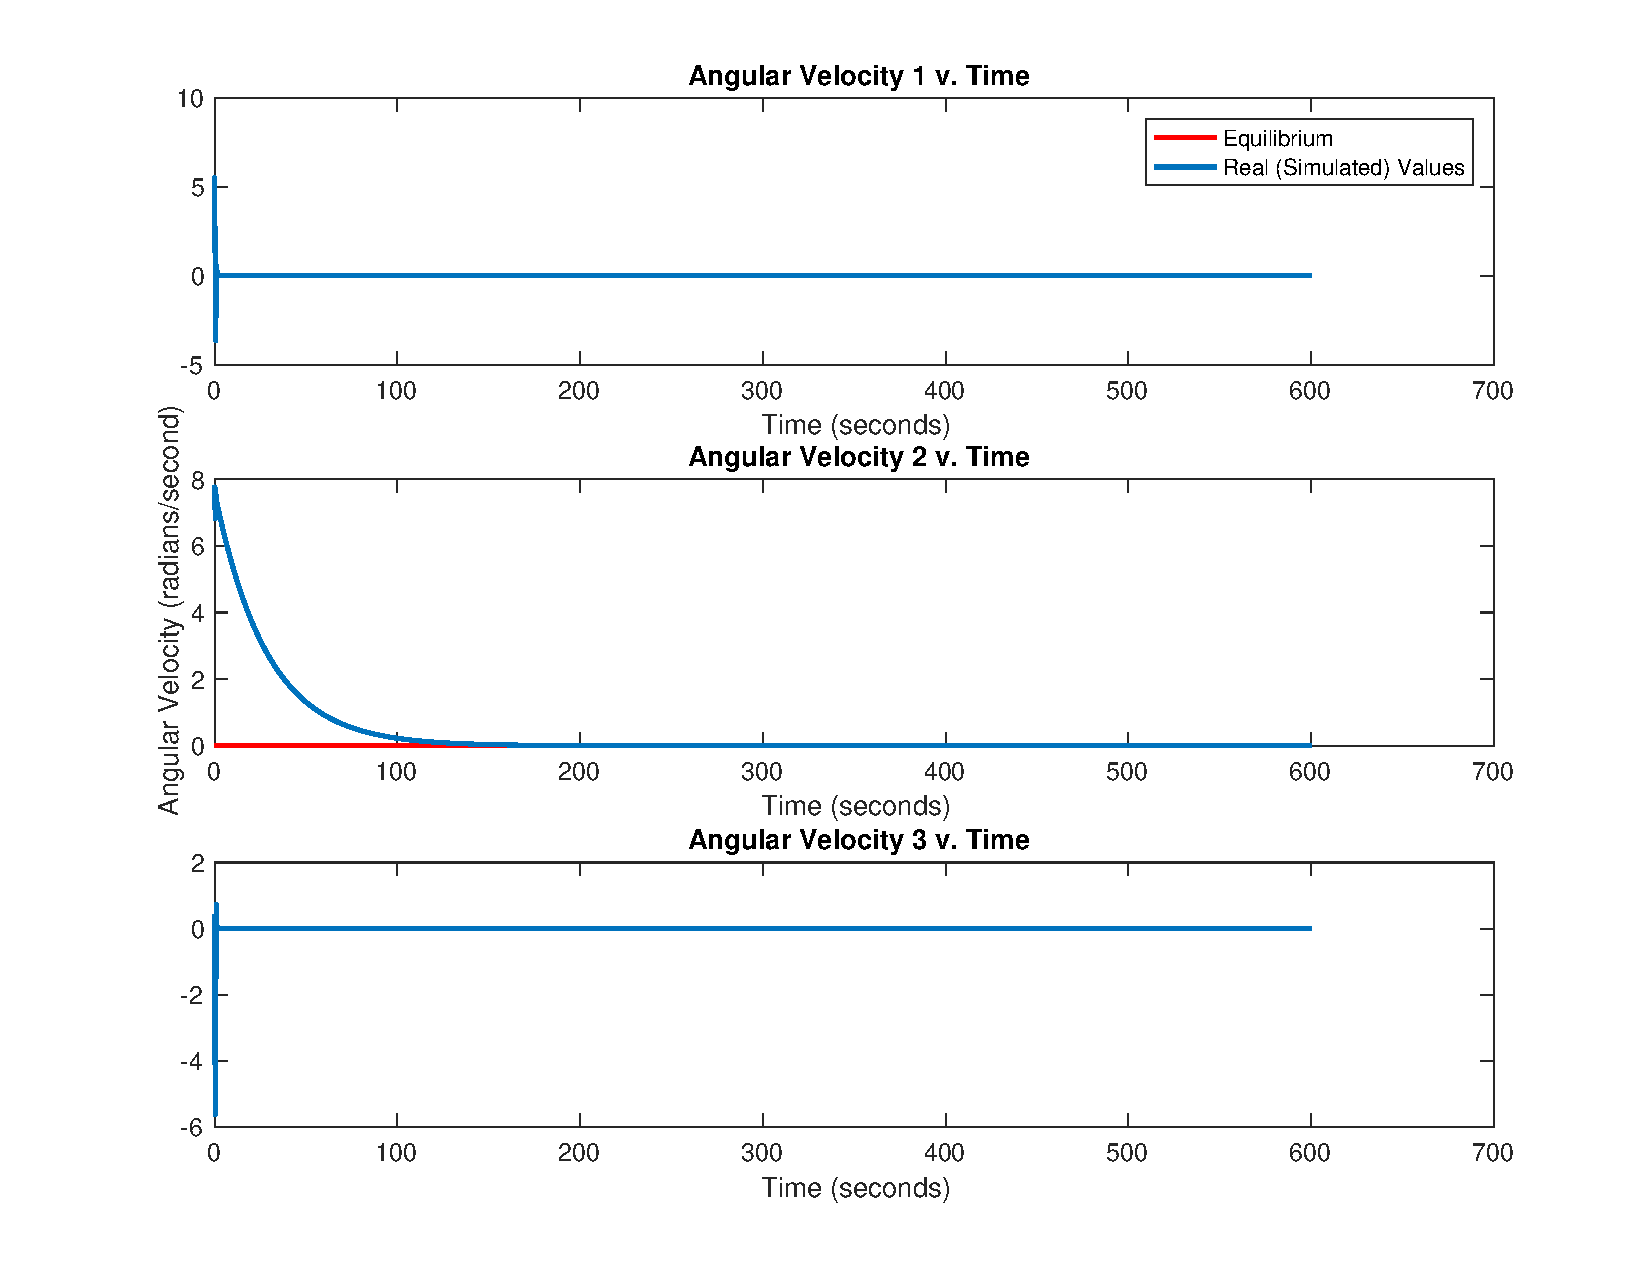
\includegraphics[width=0.5\textwidth]{rt3.pdf}}
\subfloat[]{
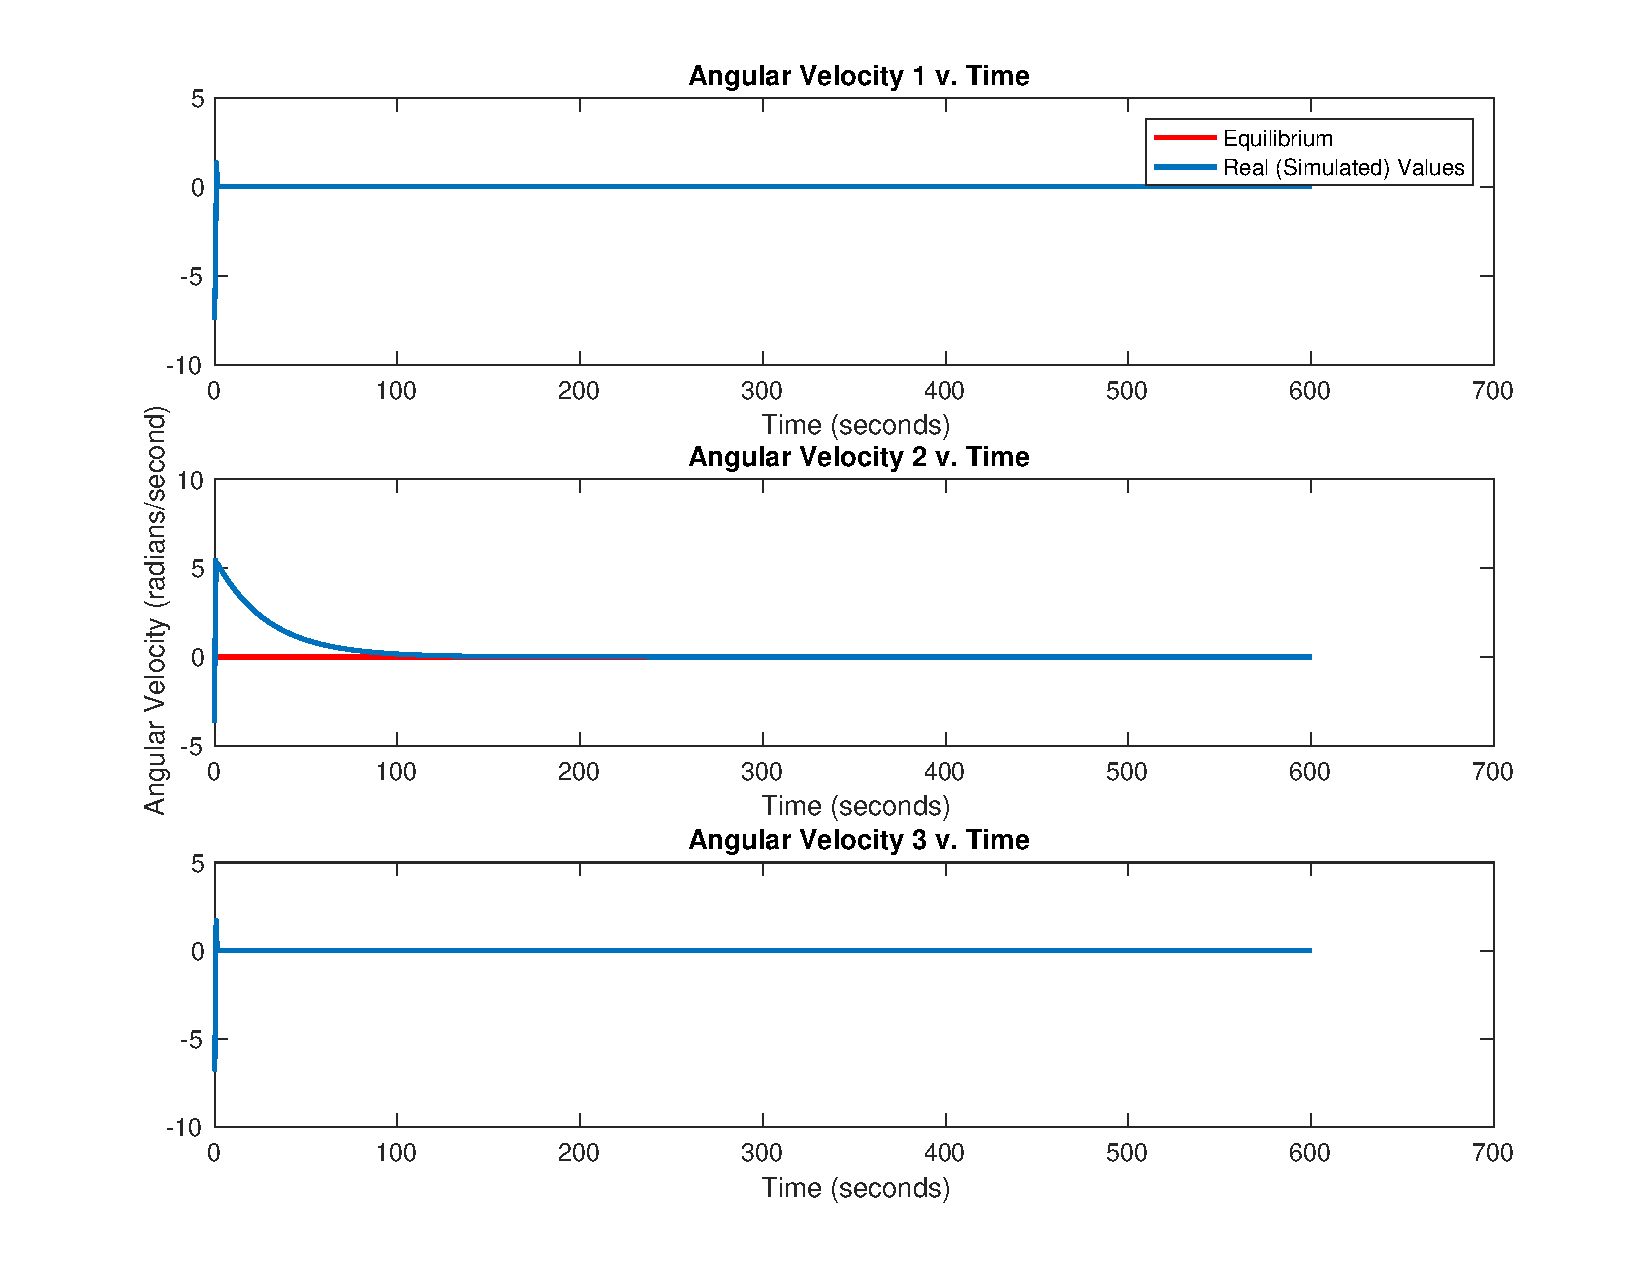
\includegraphics[width=0.5\textwidth]{r4.pdf}}
\caption{Spacecraft simulation with  $w_{0}$=[rand]}
\label{fig:8}
\end{figure}
\section{Conclusion}
DesignProblem01 simulates the rotational motion of a spacecraft given a random initial angular velocity. The goal was established such that the spacecrafts equilibrium angular velocity must be equal to Earth's angular velocity of 7.2921159e-5 \( \frac{rad}{sec} \). It was perceived that by having an equilibrium angular velocity about a single axis orthogonal to the spacecrafts orbital plane, a satellite with a tidally locked, geosynchronous orbit can be achieved. By turning the system into a state-space model, an understanding of the satellites behavior was achieved. After defining the model, a linearization of the system was computed to allow stability at the established equilibrium points. A solution with zero input was then achieved to verify the linearization was done correctly. By implementing state feedback, the system could now correct its behavior and attempt to reach equilibrium. Finally, by introducing reference tracking to the system, the satellite can be guaranteed to reach equilibrium after some time given any random initial angular velocity. 
\\
Through simulation, the desired equilibrium of ${w}_{e}$=[0 7.2921159e-5 0] is verified to be achievable. The goal of having a satellite with a tidally locked, geosynchronous orbit can be achieved. with the exception that in practice, the system would not be practical. In this simulation, there was no parameter to send the satellite back to the equilibrium position. This means that after the satellite has experienced the random angular velocity and then stabilized to the desired angular velocities, it will be orbiting, tidally locked at an angle. If the satellite were needed to be tidally locked for reasons such as communication, having the antennae point Earth for example, then the antennae will be pointing in the wrong direction. For future studies, a position correcting parameter would be implemented to allow for orientation manipulation. 
% End of document (everything after this is ignored)
\end{document}